% Options for packages loaded elsewhere
\PassOptionsToPackage{unicode}{hyperref}
\PassOptionsToPackage{hyphens}{url}
\documentclass[
  english,
  doc,floatsintext]{apa6}
\usepackage{xcolor}
\usepackage{amsmath,amssymb}
\setcounter{secnumdepth}{-\maxdimen} % remove section numbering
\usepackage{iftex}
\ifPDFTeX
  \usepackage[T1]{fontenc}
  \usepackage[utf8]{inputenc}
  \usepackage{textcomp} % provide euro and other symbols
\else % if luatex or xetex
  \usepackage{unicode-math} % this also loads fontspec
  \defaultfontfeatures{Scale=MatchLowercase}
  \defaultfontfeatures[\rmfamily]{Ligatures=TeX,Scale=1}
\fi
\usepackage{lmodern}
\ifPDFTeX\else
  % xetex/luatex font selection
\fi
% Use upquote if available, for straight quotes in verbatim environments
\IfFileExists{upquote.sty}{\usepackage{upquote}}{}
\IfFileExists{microtype.sty}{% use microtype if available
  \usepackage[]{microtype}
  \UseMicrotypeSet[protrusion]{basicmath} % disable protrusion for tt fonts
}{}
\makeatletter
\@ifundefined{KOMAClassName}{% if non-KOMA class
  \IfFileExists{parskip.sty}{%
    \usepackage{parskip}
  }{% else
    \setlength{\parindent}{0pt}
    \setlength{\parskip}{6pt plus 2pt minus 1pt}}
}{% if KOMA class
  \KOMAoptions{parskip=half}}
\makeatother
% Make \paragraph and \subparagraph free-standing
\makeatletter
\ifx\paragraph\undefined\else
  \let\oldparagraph\paragraph
  \renewcommand{\paragraph}{
    \@ifstar
      \xxxParagraphStar
      \xxxParagraphNoStar
  }
  \newcommand{\xxxParagraphStar}[1]{\oldparagraph*{#1}\mbox{}}
  \newcommand{\xxxParagraphNoStar}[1]{\oldparagraph{#1}\mbox{}}
\fi
\ifx\subparagraph\undefined\else
  \let\oldsubparagraph\subparagraph
  \renewcommand{\subparagraph}{
    \@ifstar
      \xxxSubParagraphStar
      \xxxSubParagraphNoStar
  }
  \newcommand{\xxxSubParagraphStar}[1]{\oldsubparagraph*{#1}\mbox{}}
  \newcommand{\xxxSubParagraphNoStar}[1]{\oldsubparagraph{#1}\mbox{}}
\fi
\makeatother
\usepackage{graphicx}
\makeatletter
\newsavebox\pandoc@box
\newcommand*\pandocbounded[1]{% scales image to fit in text height/width
  \sbox\pandoc@box{#1}%
  \Gscale@div\@tempa{\textheight}{\dimexpr\ht\pandoc@box+\dp\pandoc@box\relax}%
  \Gscale@div\@tempb{\linewidth}{\wd\pandoc@box}%
  \ifdim\@tempb\p@<\@tempa\p@\let\@tempa\@tempb\fi% select the smaller of both
  \ifdim\@tempa\p@<\p@\scalebox{\@tempa}{\usebox\pandoc@box}%
  \else\usebox{\pandoc@box}%
  \fi%
}
% Set default figure placement to htbp
\def\fps@figure{htbp}
\makeatother
% definitions for citeproc citations
\NewDocumentCommand\citeproctext{}{}
\NewDocumentCommand\citeproc{mm}{%
  \begingroup\def\citeproctext{#2}\cite{#1}\endgroup}
\makeatletter
 % allow citations to break across lines
 \let\@cite@ofmt\@firstofone
 % avoid brackets around text for \cite:
 \def\@biblabel#1{}
 \def\@cite#1#2{{#1\if@tempswa , #2\fi}}
\makeatother
\newlength{\cslhangindent}
\setlength{\cslhangindent}{1.5em}
\newlength{\csllabelwidth}
\setlength{\csllabelwidth}{3em}
\newenvironment{CSLReferences}[2] % #1 hanging-indent, #2 entry-spacing
 {\begin{list}{}{%
  \setlength{\itemindent}{0pt}
  \setlength{\leftmargin}{0pt}
  \setlength{\parsep}{0pt}
  % turn on hanging indent if param 1 is 1
  \ifodd #1
   \setlength{\leftmargin}{\cslhangindent}
   \setlength{\itemindent}{-1\cslhangindent}
  \fi
  % set entry spacing
  \setlength{\itemsep}{#2\baselineskip}}}
 {\end{list}}
\usepackage{calc}
\newcommand{\CSLBlock}[1]{\hfill\break\parbox[t]{\linewidth}{\strut\ignorespaces#1\strut}}
\newcommand{\CSLLeftMargin}[1]{\parbox[t]{\csllabelwidth}{\strut#1\strut}}
\newcommand{\CSLRightInline}[1]{\parbox[t]{\linewidth - \csllabelwidth}{\strut#1\strut}}
\newcommand{\CSLIndent}[1]{\hspace{\cslhangindent}#1}
\ifLuaTeX
\usepackage[bidi=basic]{babel}
\else
\usepackage[bidi=default]{babel}
\fi
% get rid of language-specific shorthands (see #6817):
\let\LanguageShortHands\languageshorthands
\def\languageshorthands#1{}
\ifLuaTeX
  \usepackage[english]{selnolig} % disable illegal ligatures
\fi
\setlength{\emergencystretch}{3em} % prevent overfull lines
\providecommand{\tightlist}{%
  \setlength{\itemsep}{0pt}\setlength{\parskip}{0pt}}
% Manuscript styling
\usepackage{upgreek}
\captionsetup{font=singlespacing,justification=justified}

% Table formatting
\usepackage{longtable}
\usepackage{lscape}
% \usepackage[counterclockwise]{rotating}   % Landscape page setup for large tables
\usepackage{multirow}		% Table styling
\usepackage{tabularx}		% Control Column width
\usepackage[flushleft]{threeparttable}	% Allows for three part tables with a specified notes section
\usepackage{threeparttablex}            % Lets threeparttable work with longtable

% Create new environments so endfloat can handle them
% \newenvironment{ltable}
%   {\begin{landscape}\centering\begin{threeparttable}}
%   {\end{threeparttable}\end{landscape}}
\newenvironment{lltable}{\begin{landscape}\centering\begin{ThreePartTable}}{\end{ThreePartTable}\end{landscape}}

% Enables adjusting longtable caption width to table width
% Solution found at http://golatex.de/longtable-mit-caption-so-breit-wie-die-tabelle-t15767.html
\makeatletter
\newcommand\LastLTentrywidth{1em}
\newlength\longtablewidth
\setlength{\longtablewidth}{1in}
\newcommand{\getlongtablewidth}{\begingroup \ifcsname LT@\roman{LT@tables}\endcsname \global\longtablewidth=0pt \renewcommand{\LT@entry}[2]{\global\advance\longtablewidth by ##2\relax\gdef\LastLTentrywidth{##2}}\@nameuse{LT@\roman{LT@tables}} \fi \endgroup}

% \setlength{\parindent}{0.5in}
% \setlength{\parskip}{0pt plus 0pt minus 0pt}

% Overwrite redefinition of paragraph and subparagraph by the default LaTeX template
% See https://github.com/crsh/papaja/issues/292
\makeatletter
\renewcommand{\paragraph}{\@startsection{paragraph}{4}{\parindent}%
  {0\baselineskip \@plus 0.2ex \@minus 0.2ex}%
  {-1em}%
  {\normalfont\normalsize\bfseries\itshape\typesectitle}}

\renewcommand{\subparagraph}[1]{\@startsection{subparagraph}{5}{1em}%
  {0\baselineskip \@plus 0.2ex \@minus 0.2ex}%
  {-\z@\relax}%
  {\normalfont\normalsize\itshape\hspace{\parindent}{#1}\textit{\addperi}}{\relax}}
\makeatother

\makeatletter
\usepackage{etoolbox}
\patchcmd{\maketitle}
  {\section{\normalfont\normalsize\abstractname}}
  {\section*{\normalfont\normalsize\abstractname}}
  {}{\typeout{Failed to patch abstract.}}
\patchcmd{\maketitle}
  {\section{\protect\normalfont{\@title}}}
  {\section*{\protect\normalfont{\@title}}}
  {}{\typeout{Failed to patch title.}}
\makeatother

\usepackage{xpatch}
\makeatletter
\xapptocmd\appendix
  {\xapptocmd\section
    {\addcontentsline{toc}{section}{\appendixname\ifoneappendix\else~\theappendix\fi: #1}}
    {}{\InnerPatchFailed}%
  }
{}{\PatchFailed}
\makeatother
\keywords{Trust in science; science knowledge; cognition; deficit model}
\usepackage{csquotes}
\usepackage{placeins} 

\usepackage{bookmark}
\IfFileExists{xurl.sty}{\usepackage{xurl}}{} % add URL line breaks if available
\urlstyle{same}
\hypersetup{
  pdftitle={Trusting but forgetting impressive science},
  pdfauthor={Jan Pfänder1, Sophie de Rouilhan2, \& Hugo Mercier2},
  pdflang={en-EN},
  pdfkeywords={Trust in science; science knowledge; cognition; deficit model},
  hidelinks,
  pdfcreator={LaTeX via pandoc}}

\title{Trusting but forgetting impressive science}
\author{Jan Pfänder\textsuperscript{1}, Sophie de Rouilhan\textsuperscript{2}, \& Hugo Mercier\textsuperscript{2}}
\date{}


\shorttitle{Trusting but forgetting impressive science}

\authornote{

We thank Kevin Chen for excellent research assistance.

Correspondence concerning this article should be addressed to Jan Pfänder. E-mail: \href{mailto:janlukas.pfaender@gmail.com}{\nolinkurl{janlukas.pfaender@gmail.com}}

}

\affiliation{\vspace{0.5cm}\textsuperscript{1} Swiss Federal Institute of Aquatic Science and Technology (Eawag), Department of Environmental Social Sciences\\\textsuperscript{2} Institut Jean Nicod, Département d'études cognitives, ENS, EHESS, PSL University, CNRS, France}

\abstract{%
Cultural beliefs and practices often spread because they appeal to existing cognitive mechanisms. Science, however, appears to be an exception. Scientific concepts are highly counterintuitive, and people know very little about science, yet it is among the most trusted institutions. Here, we test a cognitive model of trust in science that is compatible with these observations: the rational impression account. According to this account, people trust scientists because they are impressed by their findings, and this impression persists after specific knowledge has vanished. We present evidence for this model in two experiments (total n = 696) with UK participants. In Experiment 1, exposure to more impressive scientific findings led participants to think of the relevant scientists as more competent and their scientific discipline as more trustworthy. In Experiment 2, we show that participants have these impressions despite almost immediately forgetting relevant content.
}



\begin{document}
\maketitle

\section{Introduction}\label{introduction}

Scholars have suggested that culturally widespread beliefs often owe their success to their ability to tap into existing cognitive mechanisms (for a general exposition, see Sperber, 1996). This idea has been applied, for instance, to religion (Boyer, 1994; Lawson \& McCauley, 1990), fiction (Dubourg \& Baumard, 2022; Gottschall, 2012), music (Fitch, 2006), rituals (Liénard \& Boyer, 2006), or medical practices (Miton, Claidière, \& Mercier, 2015). In each case, cognitive mechanisms render some cultural elements more likely to draw our attention, be remembered, or be passed along. When a cultural element violates the expectations raised by our cognitive mechanisms, it is supposed to be only in a minimal manner that maximises attraction or memorization, as in the case minimally counter-intuitive religious beliefs (Boyer, 1994; Norenzayan, Atran, Faulkner, \& Schaller, 2006).

In these models of culture, it is the ability to produce cultural elements that people find appealing that would largely explain the status of their creators, from successful fiction authors to religious figures (see, e.g., André, Baumard, \& Boyer, 2023; Boyer, 2021; Singh, 2018). In this context, science seems to stand out as an exception. By contrast with fiction, which people (in the US) consume for several hours a day on average, consumption of science-related materials (news, popular science, etc.) is minimal, with only a small minority consuming scientific content several times a week (Funk, Gottfried, \& Mitchell, 2017). By contrast with the ``naturalness of religious ideas'' (Boyer, 1994), many researchers have pointed out the ``unnatural nature of science,'' (Wolpert, 1994; see Cromer, 1995; McCauley, 2011; Shtulman, 2017): how counterintuitive many fundamental scientific concepts are, from Newton's first law of motion (which violates our intuitions about physics, McCloskey, Caramazza, \& Green, 1980), to evolution by natural selection (which violates, inter alia, our intuitions about reproduction, Ronfard, Brown, Doncaster, \& Kelemen, 2021). Given that most people do not consume much scientific content, it is not surprising that average levels of science knowledge are very low (National Academies of Sciences, Engineering, and Medicine, 2016). What \emph{is} surprising is that, in spite of this lack of knowledge, and of the ``unnaturalness'' of much of science, people worldwide tend to trust science (Cologna et al., 2025; Wellcome Global Monitor, 2018). In the US, where survey data allows for comparison, science is among the most trusted institutions (Funk \& Kennedy, 2020).

We start by briefly reviewing existing models of trust in science, pointing out that most do not have much to say about the cognitive foundations of trust in science, being chiefly interested in explaining mistrust of science. One of these models, the deficit model, offers a potential cognitive explanation of trust in science, in that trust in science would be grounded in an understanding and knowledge of science. However, as mentioned above, this is difficult to reconcile with the fact that trust in science tends to be much higher than understanding or knowledge of science. The recently developed rational impression account of trust in science (Pfänder \& Mercier, 2025) can reconcile high levels of trust in science with lack of science knowledge and understanding. This article offers a direct experimental test of two central tenets of this rational impression account: (i) that people trust impressive science, and (ii) that they promptly forget what had impressed them.

\section{Theoretical background}\label{theoretical-background}

Much of the literature on public trust in science has focused on explaining why some people do not trust science (Bauer, Allum, \& Miller, 2007). The deficit model assumes that trust deficits among the public are due to a lack of scientific knowledge (Sturgis \& Allum, 2004). Motivated reasoning accounts argue that people reject science to maintain coherence with certain prior beliefs and worldviews (Lewandowsky \& Oberauer, 2021). Other psychological accounts highlight ideologies, conspiratorial thinking, or personality as root causes of mistrust (Hornsey \& Fielding, 2017). In the sociological literature, the alienation model suggests that mistrust in science is only one symptom of a broader alienation of people from modern institutions (Gauchat, 2011). These accounts do not attempt to explain the elevated level of public trust in science. Implicitly, they take trust in science for granted, as a normatively rational default, and focus on explaining deviations from this default.

Recently, a large survey project in 68 countries found trust in scientists to be ``moderately high'' across all countries (mean = 3.62; sd= 0.70; Scale: 1 = very low, 2 = somewhat low, 3 = neither high nor low, 4 = somewhat high, 5 = very high), with not a single country below midpoint trust (Cologna et al., 2025). This is in line with past global surveys, which found that most people trust science at least to some extent (Wellcome Global Monitor, 2018, 2020). In the US, the General Social Survey (GSS) allows to compare trust in science with trust in other institutions. Combining data from 1973 to 2022, on average 43\% of Americans say they have a great deal of confidence in the scientific community, the second highest score among 13 institutions, and surpassing religion by far (26\%)\footnote{Numbers are based on our own calculations using on the publicly available GSS cumulative data}. These surveys might still underestimate public trust in scientific knowledge: A recent study in the US found that participants almost always accepted the scientific consensus on basic, non-politicized knowledge questions (e.g.~`Are electrons are smaller than atoms?'), even those participants who said they do not trust science and who believed anti-science conspiracy theories, e.g.~that the earth is flat (Pfänder, Kerzreho, \& Mercier, 2025).

While existing accounts focus on explaining mistrust, the deficit model implicitly offers an explanation for trust: if a lack of knowledge is the main reason for a lack of trust, then knowledge should be the main cause of trust. The issue with this explanation is that, while people tend to trust science, they do not know much about it (National Academies of Sciences, Engineering, and Medicine, 2016). A recent global study on 68 countries found no association between the countries' Program for International Student Assessment (PISA) scores, and the national average trust in scientists (Cologna et al., 2025). A seminal meta analysis found that science knowledge, more generally, was only weakly correlated to attitudes towards science (Allum, Sturgis, Tabourazi, \& Brunton-Smith, 2008).

Recently, a cognitive explanation for public trust in science has been proposed: the rational impression account (Pfänder \& Mercier, 2025). According to this account, people do not need a profound understanding or detailed knowledge of science, to rationally perceive it as trustworthy. Instead, people can come to this conclusion by using basic cognitive mechanisms of information evaluation. The rational impression account comprises three such mechanisms: First, in many situations, we infer accuracy from consensus---i.e.~if something is highly consensual, it is likely to be true. The literature on the wisdom of crowds has shown that this inference is often appropriate (see e.g., Hastie \& Kameda, 2005). In non-science related contexts, it has been shown that people go even further and infer that convergent answers are likely accurate, and those who made them competent, even if they had no priors about their competence(Pfänder, De Courson, \& Mercier, 2025).

Second, we infer competence from possessing rare knowledge---if someone knows something that is difficult to know, we are impressed, and deem that individual competent. People perceive others who share valuable ideas as more competent (Altay, Majima, \& Mercier, 2020). Outside the realm of science, with trivia questions, it has been shown that people have accurate perceptions of whether something is hard to know or not, and that they use this information to infer someone's competence (Dubourg, Dheilly, Mercier, \& Morin, 2025).

Third, we are likely to forget the specific knowledge that generated our impressions of competence. Relevant evidence comes from memory research: Some research has shown that implicit memory is more stable than explicit memory (Parkin, Reid, \& Russo, 1990; e.g., Sloman, Hayman, Ohta, Law, \& Tulving, 1988). Other research has argued that memory encodes information both as ``verbatim'' details (exact words or numbers) and ``gist'' representations {[}the essence or bottom line meaning; Reyna (2021){]}, and that the verbatim details tend to fade faster than the gist (Murphy \& Shapiro, 1994). As an extreme example, patients with severe amnesia can continue to experience emotions linked to events they could not recall (Feinstein, Duff, \& Tranel, 2010). Similarly, in the case of science, people might forget the specific content of science knowledge (explicit memory, or verbatim details) they have been exposed to, but retain an abstract impression of scientists' trustworthiness (implicit memory, or gist). While this process has not been tested, evidence suggest that impression formation and knowledge retention can be quite detached: Liquin and Lombrozo (2022) found that people find some science-related explanations more satisfying than others. However, the satisfaction people felt for an explanation did not predict how well they could recall it shortly after (Liquin \& Lombrozo, 2022).

The rational impression account of trust in science can reconcile high levels of trust in science with the fact that people aren't very interested in science (it's enough that they have been exposed to science at school, even if they forget much of what they learnt), and that science is counterintuitive (a finding doesn't have to be intuitive to be impressive---to some extent, the contrary could be true, provided we believe in the finding). Moreover, it grounds trust in science in the operation of well-established cognitive mechanisms. If the general operation of these mechanisms has been studied, their specific application to scientific information and trust in science has not.

Here, we test two key predictions from the rational impression account: People trust more science they perceive as more impressive (H1, tested in Experiment 1), and they forget most of what had impressed them (H2, tested in Experiment 2).

\section{The present studies}\label{the-present-studies}



\begin{figure}
\centering
\pandocbounded{\includegraphics[keepaspectratio]{output/figures/overview-plot.pdf}}
\caption{\label{fig:overview-plot}\textbf{A.} An overview of the differences in trust, according to whether the participants had read a basic, an impressive, or another participant's recalled version of the impressive vignette. The density plots show the distributions of participants' trust scores. The dots represent model estimates, and the vertical bars the 95\% confidence intervals of the model predictions. \textbf{B.} The distribution of knowledge scores (ranging from 0\% to 100\% retained information) in the recall study of Experiment 2. Each dot corresponds to one participant. For the boxplot, the box represents the interquartile range (IQR), that is, the distance between the first and third quartiles, the center line indicates the median, and the outer lines (whiskers) extend to 1.5 times the IQR or the most extreme values within this range.}
\end{figure}

Both experiments were preregistered, and the choice of sample size was informed by power simulations. The preregistrations, along with all materials, data, and code, can be found on Open Science Framework \href{https://osf.io/j3bk4/overview}{project page} (\url{https://osf.io/j3bk4/overview}). All analyses were conducted in R (version 4.2.2) using R Studio. We used two-sided tests for all hypotheses. Unless mentioned otherwise, we report unstandardized estimates that can be interpreted in units of the original scales.

As part of this project, we conducted two additional experiments which we present in detail in the ESM. The first experiment (`Experiment 1b' in the ESM) is almost identical to Experiment 1, but suffered from a minor technical error during the implementation. Nonetheless, its findings are identical to those of Experiment 1. The second experiment (`Experiment 2b') was supposed to test the same hypothesis as Experiment 2, but the treatment---a very short distraction task---did not alter any of the outcome variables, suggesting that either the distraction task was too short, or that our outcome measure---a set of multiple-choice questions---was not sufficiently sensitive.

\section{Experiment 1}\label{experiment-1}

The goal of Experiment 1 was to test whether exposure to impressive science content enhanced people's trust in scientists and their discipline. Participants were presented with vignettes about scientific findings in the disciplines of entomology and archaeology. The impressiveness of the texts was manipulated by creating one `basic' and one `impressive' version for each of the disciplines (see Table \ref{tab:exp1-stimuli}). Impressiveness was manipulated within participants, but between disciplines: each participant was randomly assigned to see an impressive version for one discipline, and a basic version for the other discipline. We tested the following hypotheses:

H1a: After having read an impressive text about a discipline's findings, compared to when reading a basic text, participants perceive that discipline's scientists as more competent.

H1b: Across both conditions, participants who are more impressed by the text about a discipline also tend to perceive the scientists of that discipline as more competent.

H2a: After reading an impressive text about a discipline's findings, compared to when reading a basic text, participants will trust the discipline more.

H2b: Across both conditions, participants who are more impressed by the text about a discipline also tend to trust the discipline more.

The results of two research questions, about perceptions of learning and of consensus, are reported in the ESM.

\subsection{Methods}\label{methods}

\subsubsection{Participants}\label{participants}

A power simulation (see OSF) suggested that the minimum required sample size to detect a statistically significant effect for all hypotheses with a power of 0.9 is 100 participants. We therefore recruited 100 participants from the UK via Prolific. One participant failed the attention check, resulting in a final sample of 99 participants (49 female, 50 male; \(age_\text{mean}\): 42.07, \(age_\text{sd}\): 12.86, \(age_\text{median}\): 40).

\subsubsection{Procedure}\label{procedure}

After providing their consent to participate in the study and passing an attention check (see ESM), participants read a short introductory text, and then two vignettes (one basic and one impressive) about scientific findings in the disciplines of entomology and archaeology, in a randomized order. After reading each vignette, participants were asked: ``How much do you feel you've learnt about {[}human history/insects{]} by reading this text?'' {[}1 - Nothing, 2 - A bit, 3 - Some, 4 - Quite a bit, 5 - A lot{]}); ``How impressive do you think the findings of the {[}archaeologists/entomologists{]} described in the text are?'' {[}1 - Not very impressive, 2 - A bit impressive, 3 - Quite impressive, 4 - Very impressive, 5 - Extremely impressive{]}); ``Would you agree that reading this text has made you think of {[}archaeologists/entomologists{]} as more competent than you thought before?'' {[}1 - Strongly disagree, 2 - Disagree, 3 - Neither agree nor disagree, 4 - Agree, 5 - Strongly agree{]}); and ``Having read this text, would you agree that you trust the discipline of {[}archaeology/entomology{]} more than you did before?'' {[}1 - Strongly disagree, 2 - Disagree, 3 - Neither agree nor disagree, 4 - Agree, 5 - Strongly agree{]}. Finally, we asked: ``To which extent do you think the findings from the short text you just read reflect a minority or a majority opinion among archaeologists?'' {[}1 - Small minority, 2 - Minority, 3 - About half, 4 - Majority, 5 - Large majority{]}.

\subsubsection{Materials}\label{materials}

Table \ref{tab:exp1-stimuli} shows the stimuli used in Experiment 1.

\begingroup\fontsize{8}{10}\selectfont

\begin{longtable}[t]{>{\raggedright\arraybackslash}p{5em}>{\raggedright\arraybackslash}p{25em}>{\raggedright\arraybackslash}p{25em}}
\caption{\label{tab:exp1-stimuli}Stimuli of Experiment 1}\\
\toprule
 & Impressive & Basic\\
\midrule
\endfirsthead
\caption[]{\label{tab:exp1-stimuli}Stimuli of Experiment 1 \textit{(continued)}}\\
\toprule
 & Impressive & Basic\\
\midrule
\endhead

\endfoot
\bottomrule
\endlastfoot
Archeology & Archaeologists, scientists who study human history and prehistory, are able to tell, from their bones, whether someone was male or female, how old they were, and whether they suffered from a range of diseases. Archaeologists can now tell at what age someone, dead for tens of thousands of years, stopped drinking their mother’s milk, from the composition of their teeth.
Archaeologists learn about the language that our ancestors or cousins might have had. For instance, the nerve that is used to control breathing is larger in humans than in apes, plausibly because we need more fine-grained control of our breathing in order to speak. As a result, the canal containing that nerve is larger in humans than in apes – and it is also enlarged in Neanderthals.
Archaeologists can also tell, from an analysis of the tools they made, that most Neanderthals were right-handed. It’s thought that handedness is related to the evolution of language, another piece of evidence suggesting that Neanderthals likely possessed a form of language. & Archaeology is the science that studies human history and prehistory based on the analysis of objects from the past such as human bones, engravings, constructions, and various objects, from nails to bits of pots. This task requires a great deal of carefulness, because objects from the past need to often be dug out from the ground and patiently cleaned, without destroying them in the process.

Archaeologists have been able to shed light on human history in all continents, from ancient Egypt to the Incas in Peru or the Khmers in Cambodia.

Archaeologists study the paintings made by our ancestors, such as those that can be found in Lascaux, a set of caves found in the south of France that have been decorated by people at least 30000 years ago.

Archaeologists have also found remains of our more distant ancestors, showing that our species is just one among several that appeared, and then either changed or went extinct, such as Neanderthals, Homo erectus, or Homo habilis.\\
Entomology & Entomologists are the scientists who study insects. Some of them have specialized in understanding how insects perceive the world around them, and they have uncovered remarkable abilities. 

Entomologists interested in how flies’ visual perception works have used special displays to present images for much less than the blink of an eye, electrodes to record how individual cells in the flies’ brain react, and ultra-precise electron microscopy to examine their eyes. Thanks to these techniques, they have shown that some flies can perceive images that are displayed for just three milliseconds (a thousandth of a second) – about ten times shorter than a single movie frame (of which there are 24 per second). 

Entomologists who study the hair of crickets have shown that these microscopic hairs, which can be found on antenna-like organs attached to the crickets’ rear, are maybe the most sensitive organs in the animal kingdom. The researchers used extremely precise techniques to measure how the hair reacts to stimuli, such as laser-Doppler velocimetry, a technique capable of detecting the most minute of movements. They were able to show that the hair could react to changes in the motion of the air that had less energy than one particle of light, a single photon. & Entomologists are scientists who investigate insects, typically having a background in biology. They study, for example, how a swarm of bees organizes, or how ants communicate with each other. 

They also study how different insects interact with each other and their environment, whether some species are in danger of going extinct, or whether others are invasive species that need to be controlled.

Sometimes entomologists study insects by observing them in the wild, sometimes they conduct controlled experiments in laboratories, to see for example how different environmental factors change the behavior of insects, or to track exactly the same insects over a longer period of time.

An entomologist often specializes in one type of insect in order to study it in depth. For example, an entomologist who specializes in ants is called a myrmecologist.\\*
\end{longtable}
\endgroup{}

\subsection{Results and discussion}\label{results-and-discussion}

As a manipulation check, we find that participants perceived the impressive texts to be more impressive (mean = 4.01, sd = 0.87; \(\hat{b}\) = 0.81 {[}0.569, 1.048{]}, p \textless{} .001) than the basic texts (mean = 3.20, sd = 1.13).

Participants perceived scientists as more competent after having read an impressive text (H1a: \(\hat{b}_{\text{Competence}}\) = 0.50 {[}0.314, 0.676{]}, p \textless{} .001; mean = 3.76, sd = 0.90) than after having read a basic one (mean = 3.26, sd = 0.80). Pooled across both conditions, participants' impressiveness ratings were positively associated with competence: When participants reported being more impressed, they evaluated scientist's as more competent (H1b: \(\hat{b}\) = 0.41 {[}0.312, 0.502{]}, p \textless{} .001). Figure \ref{fig:overview-plot} provides an overview of the main results of both Experiment 1, and Experiment 2.

Participants also trusted a discipline more after having read an impressive text (H2a: \(\hat{b}_{\text{trust}}\) = 0.32 {[}0.17, 0.476{]}, p \textless{} .001; mean = 3.68, sd = 0.87) than after having read a basic one (mean = 3.35, sd = 0.84). Participants' impressiveness ratings were positively associated with trust when pooling across all conditions (H2b: \(\hat{b}\) = 0.30 {[}0.206, 0.385{]}, p \textless{} .001).

\section{Experiment 2}\label{experiment-2}

In Experiment 1, exposure to impressive scientific content increased trust in the relevant scientific discipline, and the perceived competence of the relevant scientists. Experiment 2 sought to test whether these perceptions were at least partly independent of being able to recall the specific content that had induced them. Experiment 2 consisted of a `recall study' and an `evaluation study.' In the recall study, each participant was assigned to read the impressive version of one of the vignettes from Experiment 1 (Table \ref{tab:exp1-stimuli}). As in Experiment 1, participants were asked about how impressed they were by the findings and whether they had changed their perception of the scientists' competence and their trust in the scientific discipline.

In line with the findings of Experiment 1, we expected participants to have increased perceptions of competence and trust in scientists after having read the impressive texts:

H1a: Participants perceive scientists as more competent after having read an impressive text about their discipline's findings.

H1b: Participants trust a discipline more after having read an impressive text about the discipline's findings.

In Experiment 2, participants were also given a recall task: They were asked to rewrite the text of the vignette they had just read, from memory. We predicted that participants would not be able to recall all the information presented in the short vignettes right after having read them (see methods section for details):

H2: Participants are not able to recall all the information of the original texts.

This hypothesis, however, only tested whether people forgot any of the content, potentially including non-impressive content. To address this issue, we asked participants to select elements of the vignettes they found impressive (see Table \ref{tab:knowledge-evaluation-grid}). We predicted that even for the subset of information that a participant said they found impressive, they forgot at least some of the content:

H3: Participants are not able to recall all the impressive information--as rated by themselves--contained in the original text.

H3 tests the hypothesis that participants immediately forget at least some of the information that has impressed them. However, it could be that participants in fact remember enough impressive information to justify the increase in perceived trust (in the discipline) and competence (in the scientists). To test whether that was the case, we conducted an evaluation study.

A new sample of participants was recruited, and they were randomly assigned to one of two conditions: In the `original impressive text' condition, participants were assigned to read one of the two impressive texts of the recall study. In the `recalled impressive text' condition, participants read one of the recall texts written by the participants of the recall study. We predicted that participants in the evaluation study would be less impressed by the texts recalled by the participants of the recall study, compared to the original impressive vignette texts (see Table \ref{tab:exp1-stimuli}) and, accordingly, would have less positive perceptions of the scientists' competence and the trustworthiness of their discipline:

H4a: The texts produced by participants of the experiment as a result of the recall task will be less impressive than the original texts, as rated by participants of the \textbf{evaluation study}.

H4b: Participants of the \textbf{evaluation study} perceive scientists as more competent after having read the original texts, compared to after having read the texts produced by participants of the experiment as a result of the recall task.

H4c: Participants of the \textbf{evaluation study} trust a discipline more after having read the original texts, compared to after having read the texts produced by participants of the experiment as a result of the recall task.

\subsection{Methods}\label{methods-1}

\subsubsection{Participants}\label{participants-1}

In a power simulation (see OSF), we varied the sample size of the recall study and effect sizes (assuming the same effect size for all hypotheses in each scenario). For all simulations, a constant evaluation study sample size of 400 participants was assumed (only relevant for H4a, b and c). The power simulation suggested that a power level of 90\% would be reached when assuming a medium effect size of 0.5 with 50 participants. Due to uncertainty about our assumptions, we recruited a sample of 203 participants for the recall study, and a sample of 406 participants for the evaluation study. Although this was not the focus of the simulation, the results showed that for a medium effect size of 0.5, a sample size of 400 for the evaluation study yielded statistical power of greater than 90\% for all hypotheses based on this sample (H4a, b and c). All participants were from the UK, recruited via Prolific, and paid to complete the experiment.

The final sample comprised 198 participants (four failed attention checks; 99 female, 99 male; \(age_\text{mean}\): 42.65, \(age_\text{sd}\): 15.55, \(age_\text{median}\): 40) for the recall study, and 399 participants for the evaluation study (seven failed attention checks; 201 female, 198 male; \(age_\text{mean}\): 41.71, \(age_\text{sd}\): 13.48, \(age_\text{median}\): 40).

\subsubsection{Procedure}\label{procedure-1}

\paragraph{Recall study}\label{recall-study}

In the recall study, after having consented to take part in the study and passing an attention check (see ESM), participants read the impressive version of one of the vignettes from Experiment 1 (Table \ref{tab:exp1-stimuli}). After reading the text, as in Experiment 1, participants were asked about changes in their perception of the scientists' competence, and trust in the scientists' discipline. They were also asked about the impressiveness of the text they read. The order of these questions was randomized.

Next, as an open-ended question, participants were asked to recall as much information as they could of the texts they had just read. They were told that their texts would be read by future participants. To further motivate participants, they were also told that they would get a bonus for recalling (without external aids) accurate information. They were not told how much that bonus would be. We paid them 5p per point gained in the recall task (see methods for how these points were assigned). This way, participants could reach a maximum bonus of 0.8 pound for archaeology (0.05p x 2 points x 8 content elements) and 0.7 pound (0.05p x 2 points x 7 content elements) for entomology. After that, participants were presented with the evaluation grid that we used to assess the open answers from the recall task (see Table \ref{tab:knowledge-evaluation-grid}). For each knowledge element, we asked participants to indicate whether they found it impressive or not (``Do you think this piece of information is impressive?'' {[}Yes; No{]}). At the end of the recall study, participants were asked about their education level.

\paragraph{Evaluation study}\label{evaluation-study}

After consenting to taking part in the study and passing an attention check (see ESM), participants read either one of the original vignettes, or a text produced as part of the recall task from the recall study. For those participants assigned to read a recall text, the text was randomly sampled (with replacement) from a pool of recall answers. Orthographic and grammatical mistakes in these texts were corrected with the help of ChatGPT beforehand. We had preregistered to sample among all recall answers from participants of the recall study. However, checking recall scores after the recall study and before launching the evaluation study, we found them to be very low on average (see ESM section \ref{above-median}). To avoid having the answers of less motivated participants in our sample, we decided to only select answers that scored at least as well as the median in the recall measure of the evaluation study. This selection is conservative in that it makes it harder to confirm our predictions under H4.

After reading the text, just as in the recall study, participants were asked about changes in their perception of the scientists' competence, trust in the scientists' discipline, and the impressiveness of the text they read. The order of these questions was randomized. Finally, participants were asked about their education level.

\subsubsection{Materials}\label{materials-1}

For Experiment 2, besides the texts recalled by the participants of the recall study, the impressive version of the stimuli used in Experiment 1 was used (see Table \ref{tab:exp1-stimuli}).

\begin{longtable}[t]{>{\raggedright\arraybackslash}p{20em}>{\raggedright\arraybackslash}p{20em}}
\caption{\label{tab:knowledge-evaluation-grid}Recall evaluation grid}\\
\toprule
Archaeology & Entomology\\
\midrule
1. Archaeologists can determine whether someone was male or female from their bones. & 1. Entomologists use special displays to present images to flies for extremely short periods (less than the blink of an eye).\\
2. Archaeologists can determine how old someone was from their bones. & 2. Entomologists can record how individual cells in flies’ brains react using electrodes.\\
3. Archaeologists can determine whether someone suffered from a range of diseases from their bones. & 3. Entomologists use ultra-precise electron microscopy to examine flies’ eyes.\\
4. Archaeologists can determine at what age someone stopped drinking their mother’s milk, based on the composition of their teeth. & 4. Some flies can perceive images displayed for just three milliseconds. This duration is about ten times shorter than a single movie frame.\\
5. The nerve controlling breathing is larger in humans than in apes. The canal containing that nerve is also larger in humans and Neanderthals than in apes. & 5. Crickets have microscopic hairs situated on antenna-like organs at their rear.\\
\addlinespace
6. The fact that the nerve controlling breathing is larger in humans is possibly due to the need for fine-grained control of breathing to speak. & 6. Crickets' hairs are possibly the most sensitive organs in the animal kingdom. They react to changes in air motion with less energy than one photon.\\
7. Archaeologists determined that most Neanderthals were right-handed, based on analysis of Neanderthals’ tools. & 7. Entomologists measured how cricket hairs react to stimuli, using laser-Doppler velocimetry, which can detect extremely minute movements.\\
8. Handedness is thought to be related to the evolution of language. This suggests that Neanderthals likely possessed a form of language. & \\
\bottomrule
\multicolumn{2}{l}{\rule{0pt}{1em}\textit{Note: }}\\
\multicolumn{2}{l}{\rule{0pt}{1em}For each knowledge element, participants could score a maximum of two points.}\\
\end{longtable}

\paragraph{Recall}\label{recall}

As shown in Table \ref{tab:knowledge-evaluation-grid}, the texts were divided into a series of knowledge elements. For each participant, the extent to which they recalled each of the different elements was coded. A recall score based on how many of these elements they mentioned in their open-ended answer was then calculated.

The coding was done with the help of ChatGPT (see ESM section \ref{gpt-prompt} for the exact prompt). The instructions were: to code 0 if a piece of knowledge was not mentioned or was mentioned with significant errors (e.g., writing ``the nerve controlling fine hand movement is bigger in humans'' instead of ``the nerve controlling breathing is bigger in humans''); to code 1 if the piece of knowledge was mentioned, but some important elements were missing (e.g., writing ``Archaeologists can determine at what age someone stopped drinking their mother's milk'' instead of ``Archaeologists can determine at what age someone stopped drinking their mother's milk from the composition of their teeth''), and/or there were some mistakes (e.g., writing ``Archaeologists can determine at what age someone stopped drinking their mother's milk, based on the bones'' instead of ``Archaeologists can determine at what age someone stopped drinking their mother's milk based on the teeth''); to code 2 if the piece of knowledge was mentioned with all the main content, even if the participant had not used the precise technical words (e.g., ``neanderthals,'' ``laser-Doppler velocimetry'') or had changed the phrasing in other ways. These instructions were intended to produce relatively generous recall scores.

Since the two vignettes contained a different number of total knowledge elements according to our evaluation grid (8 for archaeology, 7 for entomology), we used a relative measure for the final recall score, namely the share of obtained points among all possible points (possible range from 0 to 1, below the results are presented in percentages recalled for clarity). Practically, for all tests on recall, we computed a forgetting score (1-recall score), and tested whether it was statistically significantly different from zero.

To validate the scores assigned by ChatGPT, they were compared to scores assigned by two human coders for a subsample of 80 randomly chosen texts (half on archaeology, half on entomology). The human coders were unaware of the study context and the hypotheses. They were provided with the prompt given to ChatGPT. To measure the agreement between ChatGPT and the human coders, we calculated an intraclass correlation coefficient (ICC) for two-way designs with random raters (Ten Hove, Jorgensen, \& Ark, 2024). Following the guidelines in Heyman, Lorber, Eddy, and West (2014), we preregistered taking 0.7 as a threshold for acceptable reliability. In our sample, we observe an ICC of 0.84 (\(se\) = 0.03). Human coders and ChatGPT, on average, assigned exactly the same score in 72.9\% of all rating instances (compared to 73.5\% of exact agreement between the two human coders). Following our preregistration, we consider the high agreement as suggested by the ICC a validation of the use of ChatGPT.

\paragraph{Recall of impressive items}\label{recall-of-impressive-items}

After giving their post-recall evaluation of scientists' competence and trust in the discipline, participants were presented with the evaluation grid shown in Table \ref{tab:knowledge-evaluation-grid} for the respective discipline they had been randomized to see. For each element in the evaluation grid, they were asked whether they found it impressive or not. Then, for each participant, the recall score was computed just as described above, but only on the subset of those elements they had subjectively rated as impressive.

\subsection{Results and discussion}\label{results-and-discussion-1}

\subsubsection{Recall study}\label{recall-study-1}

First, as a kind of validation check, we note that most participants declared finding all knowledge elements to be impressive (\(mean_{\text{Archeology}}\) = 7.04, \(median_{\text{Archeology}}\) = 8, number of knowledge elements = 8; \(mean_{\text{Entomology}}\) = 6.39, \(median_{\text{Entomology}}\) = 7, number of knowledge elements = 7).

For the first set of hypotheses, we tested whether the average scores for perceived change in competence and trust were significantly different from their respective scale midpoints (which corresponds to no change in perception). We first tested the outcome variables' distributions for normality, using a Shapiro-Wilk test. In all cases, this test suggested that the data is considered non-normally distributed (p \textless{} 0.05). Following the preregistration, we therefore did not run a default one-sample t-test, but used a Wilcoxon signed-rank test instead. H1a and H1b were both supported: After having read an impressive text about the findings of a scientific discipline, participants saw the scientists as more competent (H1a: median = 4, W = 12,388.50, p \textless{} .001), and their discipline as more trustworthy (H1b: median = 4, W = 9,714.50, p \textless{} .001).

Despite having been impressed, a first descriptive analysis suggested that participants seemed to recall only very little information (\(mean\) = 32\%, \(sd\) = 23\%, \(median\) = 29\%). Given these low average scores, we opted for a more conservative approach to testing H2 and H3: We defined the median as a cut-off and selected only the 50\% of participants who had the highest recall scores, removing participants who may have put in less effort. Since we hypothesized that participants would forget content, this selection made it less likely that the hypotheses would be confirmed. Even for the 50\% participants with the best recall, both hypotheses were supported: Participants did not perfectly recall all information (H2: median = 0.43, W = 5778, p \textless{} .001) and they did not recall all information contained in the elements they judged as impressive themselves (H3: median = 0.43, W = 5778, p \textless{} .001)\footnote{The two median values for all information and for the subset of impressive information are not not exactly the same, but very similar, because participants rated most knowledge elements as impressive, making the general recall score and the recall score for impressive elements very similar.}.

\subsubsection{Evaluation study}\label{evaluation-study-1}

For H4a, b and c, trust, competence and impressiveness ratings were compared between the `original impressive text' and the `recalled impressive text' conditions of the evaluation study using independent sample t-tests. Participants who read one of the two original impressive texts reported being more impressed (H4a: \(\hat{b}_{\text{Impressiveness}}\) = 0.39, t = 5.41, p \textless{} .001; \(mean_{\text{Original text}}\) = 4.50, \(mean_{\text{Recalled text}}\) = 4.11), rated the scientists of the respective discipline as more competent (H4b: \(\hat{b}_{\text{Competence}}\) = 0.27, t = 3.07, p = 0.002; \(mean_{\text{Original text}}\) = 3.88, \(mean_{\text{Recalled text}}\) = 3.61), and had more trust in the respective discipline (H4c: \(\hat{b}_{\text{Trust}}\) = 0.27, t = 3.40, p \textless{} .001; \(mean_{\text{Original text}}\) = 3.81, \(mean_{\text{Recalled text}}\) = 3.54) than participants who read one of the texts of the recall task.

\section{Discussion}\label{discussion}

From a perspective of cultural evolution, the fact that people around the globe tend to trust science is puzzling: people aren't very interested in science, they struggle to understand its counterintuitive concepts, and yet they tend to trust it. A common explanation of trust in science, the deficit model, postulates that trust in science is grounded in knowledge and understanding---yet, people's science literacy is generally low and at best weakly correlated to trust in science.

Recently, a cognitive account of trust in science has been proposed to make sense of this puzzle: the rational impression account. According to this account, people are impressed by science---in particular when they encounter it in their education---which leads them to trust it, but they then forget most of what they've learnt. In two experiments, we tested two central predictions of this account. Experiment 1 showed that participants perceived some scientific findings as more impressive than others. Exposure to the more impressive findings lead people to think of scientists as more competent and to trust science more. Experiment 2 showed that these impressions are formed even though participants forget most specific knowledge---including knowledge that can be assumed to have generated the impressions---almost immediately after reading it.

The present findings have practical implications: for people to generate positive impressions of science, they need to be exposed to science. This stresses the vital role of science communication and education in forming trust in science. The relationship between science communication and trust in science has already been explored in depth (e.g., Weingart \& Guenther, 2016; for a recent review see König et al., 2023), but we believe the rational impression account tested here makes a useful contribution. In particular, it suggests that, even though more understanding of the underlying methods is always preferable (König et al., 2023), even a relatively superficial exposure to impressive findings can bolster trust in science. An important caveat is that impressive findings that haven't yet gained the approval of the community might be particularly likely to backfire if people learn they have been disproven (on the importance of presenting a measure of consensus alongside scientific information, see König et al., 2023).

The present experiments have a number of limitations: First, we did not determine which features exactly made some scientific findings more impressive than others to the participants. Uncovering these features would be both of theoretical and practical interest.

Second, in Experiment 2, we had to rely on an imperfect research design for testing whether impressions persisted more than specific knowledge. However, we believe that the study still presents convincing evidence that participants forgot some---or most of---the knowledge that generated their impressions, even immediately after forming the impressions. Two lines of evidence from Experiment 2 support this argument: First, the participants of the recall study rated the impressiveness of different passages after their recall. Even when looking only at the subjective sample of impressive information for each participant, they still forgot most of it. Second, a validation study with a different set of participants found that these participants rated the recalled texts from participants of the recall study as less impressive than the original impressive texts. If the participants of the recalled texts had only forgotten irrelevant bits of information, but not impressive bits, the expectation would have been no difference.

As a third limitation, our studies were conducted on convenience samples recruited in a single country (the UK). Fourth, the studies covered a very short time frame. While we can show that participants almost immediately forget about impressive content, it is not clear from our study for how long the impressions persist (although in other contexts impressions formed on the basis of a much more superficial exposure have been shown to last for months, Gunaydin, Selcuk, \& Zayas, 2017). Future studies could extend our findings to other populations and to longer time frames.

Besides providing support for the rational account of trust in science, we hope that our findings, and the research question that prompted them, will draw more research to the grounding of trust in science in cultural evolution.

\subsubsection{Data availability}\label{data-availability}

Data for all experiments and the simulations is available on the OSF project page (\url{https://osf.io/j3bk4/overview}). Note that on the project page, all materials related to what is referred to as ``Experiment 1'' in this paper are stored under ``experiment\_2'', and all materials related to ``Experiment 2'' in this paper are stored under ``experiment\_4''. This numbering is due to the original order in which experiments for this project were conducted. For a detailed report on the other experiments conducted as part of this project, see the ESM.

\subsubsection{Code availability}\label{code-availability}

The code used to create all results (including tables and figures) of this manuscript is also available on the OSF project page (\url{https://osf.io/j3bk4/overview}).

\subsubsection{Competing interest}\label{competing-interest}

The authors declare having no competing interests.

\FloatBarrier

\section{References}\label{references}

\phantomsection\label{refs}
\begin{CSLReferences}{1}{0}
\bibitem[\citeproctext]{ref-allumScienceKnowledgeAttitudes2008}
Allum, N., Sturgis, P., Tabourazi, D., \& Brunton-Smith, I. (2008). Science knowledge and attitudes across cultures: a meta-analysis. \emph{Public Understanding of Science}, \emph{17}(1), 35--54. \url{https://doi.org/10.1177/0963662506070159}

\bibitem[\citeproctext]{ref-altayItMyIdea2020}
Altay, S., Majima, Y., \& Mercier, H. (2020). It's my idea! Reputation management and idea appropriation. \emph{Evolution and Human Behavior}, \emph{41}(3), 235--243. \url{https://doi.org/10.1016/j.evolhumbehav.2020.03.004}

\bibitem[\citeproctext]{ref-andreCulturalEvolutionProducers2023}
André, J.-B., Baumard, N., \& Boyer, P. (2023). Cultural evolution from the producers{'} standpoint. \emph{Evolutionary Human Sciences}, \emph{5}, e25. \url{https://doi.org/10.1017/ehs.2023.20}

\bibitem[\citeproctext]{ref-bauerWhatCanWe2007}
Bauer, M. W., Allum, N., \& Miller, S. (2007). What can we learn from 25 years of PUS survey research? Liberating and expanding the agenda. \emph{Public Understanding of Science}, \emph{16}(1), 79--95. \url{https://doi.org/10.1177/0963662506071287}

\bibitem[\citeproctext]{ref-boyerNaturalnessReligiousIdeas1994}
Boyer, P. (1994). \emph{The naturalness of religious ideas: A cognitive theory of religion}. Berkeley: University of California Press.

\bibitem[\citeproctext]{ref-boyerDerivingFeaturesReligions2021}
Boyer, P. (2021). Deriving Features of Religions in the Wild: How Communication and Threat-Detection May Predict Spirits, Gods, Witches, and Shamans. \emph{Human Nature}, \emph{32}(3), 557--581. \url{https://doi.org/10.1007/s12110-021-09410-y}

\bibitem[\citeproctext]{ref-colognaTrustScientistsTheir2025}
Cologna, V., Mede, N. G., Berger, S., Besley, J., Brick, C., Joubert, M., \ldots{} Zwaan, R. A. (2025). Trust in scientists and their role in society across 68 countries. \emph{Nature Human Behaviour}, 1--18. \url{https://doi.org/10.1038/s41562-024-02090-5}

\bibitem[\citeproctext]{ref-cromerUncommonSenseHeretical1995}
Cromer, A. H. (1995). \emph{Uncommon Sense: The Heretical Nature of Science} (1st ed). Oxford: Oxford University Press, Incorporated.

\bibitem[\citeproctext]{ref-dubourgWhyImaginaryWorlds2022}
Dubourg, E., \& Baumard, N. (2022). Why imaginary worlds? The psychological foundations and cultural evolution of fictions with imaginary worlds. \emph{Behavioral and Brain Sciences}, \emph{45}, e276. \url{https://doi.org/10.1017/S0140525X21000923}

\bibitem[\citeproctext]{ref-dubourgUsingNestedStructure2025}
Dubourg, E., Dheilly, T., Mercier, H., \& Morin, O. (2025). Using the Nested Structure of Knowledge to Infer What Others Know. \emph{Psychological Science}, \emph{36}(6), 443--450. \url{https://doi.org/10.1177/09567976251339633}

\bibitem[\citeproctext]{ref-feinsteinSustainedExperienceEmotion2010}
Feinstein, J. S., Duff, M. C., \& Tranel, D. (2010). Sustained experience of emotion after loss of memory in patients with amnesia. \emph{Proceedings of the National Academy of Sciences}, \emph{107}(17), 7674--7679. \url{https://doi.org/10.1073/pnas.0914054107}

\bibitem[\citeproctext]{ref-fitchBiologyEvolutionMusic2006}
Fitch, W. T. (2006). The biology and evolution of music: A comparative perspective. \emph{Cognition}, \emph{100}(1), 173--215. \url{https://doi.org/10.1016/j.cognition.2005.11.009}

\bibitem[\citeproctext]{ref-funkScienceNewsInformation2017}
Funk, C., Gottfried, J., \& Mitchell, A. (2017). \emph{Science news and information today}. Retrieved from \url{https://www.pewresearch.org/science/2017/09/20/science-news-and-information-today/}

\bibitem[\citeproctext]{ref-funkPublicConfidenceScientists2020}
Funk, C., \& Kennedy, B. (2020). \emph{Public confidence in scientists has remained stable for decades}.

\bibitem[\citeproctext]{ref-gauchatCulturalAuthorityScience2011}
Gauchat, G. (2011). The cultural authority of science: Public trust and acceptance of organized science. \emph{Public Understanding of Science}, \emph{20}(6), 751--770. \url{https://doi.org/10.1177/0963662510365246}

\bibitem[\citeproctext]{ref-gottschallStorytellingAnimalHow2012}
Gottschall, J. (2012). \emph{The Storytelling Animal: How Stories Make Us Human}. Boston: Houghton Mifflin Harcourt.

\bibitem[\citeproctext]{ref-gunaydinImpressionsBasedPortrait2017}
Gunaydin, G., Selcuk, E., \& Zayas, V. (2017). Impressions Based on a Portrait Predict, 1-Month Later, Impressions Following a Live Interaction. \emph{Social Psychological and Personality Science}, \emph{8}(1), 36--44. \url{https://doi.org/10.1177/1948550616662123}

\bibitem[\citeproctext]{ref-hastieRobustBeautyMajority2005}
Hastie, R., \& Kameda, T. (2005). The Robust Beauty of Majority Rules in Group Decisions. \emph{Psychological Review}, \emph{112}(2), 494--508. \url{https://doi.org/10.1037/0033-295X.112.2.494}

\bibitem[\citeproctext]{ref-heymanBehavioralObservationCoding2014}
Heyman, R. E., Lorber, M. F., Eddy, J. M., \& West, T. V. (2014). \emph{Behavioral observation and coding} (C. M. Judd \& H. T. Reis, Eds.). Cambridge: Cambridge University Press. \url{https://doi.org/10.1017/CBO9780511996481.018}

\bibitem[\citeproctext]{ref-hornseyAttitudeRootsJiu2017a}
Hornsey, M. J., \& Fielding, K. S. (2017). Attitude roots and Jiu Jitsu persuasion: Understanding and overcoming the motivated rejection of science. \emph{American Psychologist}, \emph{72}(5), 459--473. \url{https://doi.org/10.1037/a0040437}

\bibitem[\citeproctext]{ref-konigHowCommunicateScience2023}
König, L. M., Altenmüller, M. S., Fick, J., Crusius, J., Genschow, O., \& Sauerland, M. (2023). \emph{How to communicate science to the public? Recommendations for effective written communication derived from a systematic review}. \url{https://doi.org/10.31234/osf.io/cwbrs}

\bibitem[\citeproctext]{ref-lawsonRethinkingReligionConnecting1990}
Lawson, E. T., \& McCauley, R. N. (1990). \emph{Rethinking religion: Connecting cognition and culture}. Cambridge {[}England{]} ; New York: Cambridge University Press.

\bibitem[\citeproctext]{ref-lewandowskyWorldviewmotivatedRejectionScience2021}
Lewandowsky, S., \& Oberauer, K. (2021). Worldview-motivated rejection of science and the norms of science. \emph{Cognition}, \emph{215}, 104820. \url{https://doi.org/10.1016/j.cognition.2021.104820}

\bibitem[\citeproctext]{ref-lienardWhenceCollectiveRituals2006}
Liénard, P., \& Boyer, P. (2006). Whence Collective Rituals? A Cultural Selection Model of Ritualized Behavior. \emph{American Anthropologist}, \emph{108}(4), 814--827. \url{https://doi.org/10.1525/aa.2006.108.4.814}

\bibitem[\citeproctext]{ref-liquinMotivatedLearnAccount2022}
Liquin, E. G., \& Lombrozo, T. (2022). Motivated to learn: An account of explanatory satisfaction. \emph{Cognitive Psychology}, \emph{132}, 101453. \url{https://doi.org/10.1016/j.cogpsych.2021.101453}

\bibitem[\citeproctext]{ref-mccauleyWhyReligionNatural2011a}
McCauley, R. N. (2011). \emph{Why religion is natural and science is not}. Oxford University Press.

\bibitem[\citeproctext]{ref-mccloskeyCurvilinearMotionAbsence1980}
McCloskey, M., Caramazza, A., \& Green, B. (1980). Curvilinear Motion in the Absence of External Forces: Naïve Beliefs About the Motion of Objects. \emph{Science}, \emph{210}(4474), 1139--1141. \url{https://doi.org/10.1126/science.210.4474.1139}

\bibitem[\citeproctext]{ref-mitonUniversalCognitiveMechanisms2015}
Miton, H., Claidière, N., \& Mercier, H. (2015). Universal cognitive mechanisms explain the cultural success of bloodletting. \emph{Evolution and Human Behavior}, \emph{36}(4), 303--312. \url{https://doi.org/10.1016/j.evolhumbehav.2015.01.003}

\bibitem[\citeproctext]{ref-murphyForgettingVerbatimInformation1994}
Murphy, G. L., \& Shapiro, A. M. (1994). Forgetting of verbatim information in discourse. \emph{Memory \& Cognition}, \emph{22}(1), 85--94. \url{https://doi.org/10.3758/BF03202764}

\bibitem[\citeproctext]{ref-nationalacademiesofsciencesengineeringandmedicineScienceLiteracyConcepts2016}
National Academies of Sciences, Engineering, and Medicine. (2016). \emph{Science Literacy: Concepts, Contexts, and Consequences} (C. E. Snow \& K. A. Dibner, Eds.). Washington, D.C.: National Academies Press. \url{https://doi.org/10.17226/23595}

\bibitem[\citeproctext]{ref-norenzayanMemoryMysteryCultural2006}
Norenzayan, A., Atran, S., Faulkner, J., \& Schaller, M. (2006). Memory and Mystery: The Cultural Selection of Minimally Counterintuitive Narratives. \emph{Cognitive Science}, \emph{30}(3), 531--553. \url{https://doi.org/10.1207/s15516709cog0000_68}

\bibitem[\citeproctext]{ref-parkinDifferentialNatureImplicit1990}
Parkin, A. J., Reid, T. K., \& Russo, R. (1990). On the differential nature of implicit and explicit memory. \emph{Memory \& Cognition}, \emph{18}(5), 507--514. \url{https://doi.org/10.3758/BF03198483}

\bibitem[\citeproctext]{ref-pfanderHowWiseCrowd2025}
Pfänder, J., De Courson, B., \& Mercier, H. (2025). How wise is the crowd: Can we infer people are accurate and competent merely because they agree with each other? \emph{Cognition}, \emph{255}, 106005. \url{https://doi.org/10.1016/j.cognition.2024.106005}

\bibitem[\citeproctext]{ref-pfanderQuasiuniversalAcceptanceBasic2025b}
Pfänder, J., Kerzreho, L., \& Mercier, H. (2025). Quasi-universal acceptance of basic science in the United States. \emph{Public Understanding of Science}, 09636625251364407. \url{https://doi.org/10.1177/09636625251364407}

\bibitem[\citeproctext]{ref-pfanderRationalImpressionAccount2025a}
Pfänder, J., \& Mercier, H. (2025). \emph{The rational impression account of trust in science}. \url{https://doi.org/10.31234/osf.io/nwka2_v1}

\bibitem[\citeproctext]{ref-reynaScientificTheoryGist2021}
Reyna, V. F. (2021). A scientific theory of gist communication and misinformation resistance, with implications for health, education, and policy. \emph{Proceedings of the National Academy of Sciences}, \emph{118}(15), e1912441117. \url{https://doi.org/10.1073/pnas.1912441117}

\bibitem[\citeproctext]{ref-ronfardInhibitingIntuitionScaffolding2021}
Ronfard, S., Brown, S., Doncaster, E., \& Kelemen, D. (2021). Inhibiting intuition: Scaffolding children's theory construction about species evolution in the face of competing explanations. \emph{Cognition}, \emph{211}, 104635. \url{https://doi.org/10.1016/j.cognition.2021.104635}

\bibitem[\citeproctext]{ref-shtulmanScienceblindWhyOur2017}
Shtulman, A. (2017). \emph{Scienceblind: why our intuitive theories about the world are so often wrong}. New York: Basic Books.

\bibitem[\citeproctext]{ref-singhCulturalEvolutionShamanism2018}
Singh, M. (2018). The cultural evolution of shamanism. \emph{Behavioral and Brain Sciences}, \emph{41}, e66. \url{https://doi.org/10.1017/S0140525X17001893}

\bibitem[\citeproctext]{ref-slomanForgettingPrimedFragment1988}
Sloman, S. A., Hayman, C. A., Ohta, N., Law, J., \& Tulving, E. (1988). Forgetting in primed fragment completion. \emph{Journal of Experimental Psychology: Learning, Memory, and Cognition}, \emph{14}(2), 223.

\bibitem[\citeproctext]{ref-sperberExplainingCultureNaturalistic1996}
Sperber, D. (1996). \emph{Explaining culture: A naturalistic approach}. Oxford, UK ; Cambridge, Mass: Blackwell.

\bibitem[\citeproctext]{ref-sturgisScienceSocietyReEvaluating2004}
Sturgis, P., \& Allum, N. (2004). Science in Society: Re-Evaluating the Deficit Model of Public Attitudes. \emph{Public Understanding of Science}, \emph{13}(1), 55--74. \url{https://doi.org/10.1177/0963662504042690}

\bibitem[\citeproctext]{ref-tenhoveUpdatedGuidelinesSelecting2024}
Ten Hove, D., Jorgensen, T. D., \& Ark, L. A. van der. (2024). Updated guidelines on selecting an intraclass correlation coefficient for interrater reliability, with applications to incomplete observational designs. \emph{Psychological Methods}, \emph{29}(5), 967--979. \url{https://doi.org/10.1037/met0000516}

\bibitem[\citeproctext]{ref-weingartScienceCommunicationIssue2016}
Weingart, P., \& Guenther, L. (2016). Science communication and the issue of trust. \emph{Journal of Science Communication}, \emph{15}(05), C01. \url{https://doi.org/10.22323/2.15050301}

\bibitem[\citeproctext]{ref-wellcomeglobalmonitorWellcomeGlobalMonitor2018}
Wellcome Global Monitor. (2018). \emph{Wellcome Global Monitor 2018}. Retrieved from \url{https://wellcome.org/reports/wellcome-global-monitor/2018}

\bibitem[\citeproctext]{ref-wellcomeglobalmonitorWellcomeGlobalMonitor2020}
Wellcome Global Monitor. (2020). \emph{Wellcome Global Monitor 2020: Covid-19}. Retrieved from \url{https://wellcome.org/reports/wellcome-global-monitor-covid-19/2020}

\bibitem[\citeproctext]{ref-wolpertUnnaturalNatureScience1994}
Wolpert, L. (1994). \emph{The unnatural nature of science}. Cambridge, Mass: Harvard University Press.

\end{CSLReferences}

\newpage

\appendix


\section{Chat GPT Prompt for Experiment 2}\label{gpt-prompt}

\FloatBarrier

We provided ChatGPT with the evaluation grid (Table \ref{tab:knowledge-evaluation-grid}) and the following prompt:

\begin{quote}
\textbf{Prompt ChatGPT}: \emph{``In an experiment, participants read the following vignette : {[}\ldots{]}. Then, participants are asked to write what they recall from the vignette. Evaluate whether the following piece of information is included in the participant's text : {[}\ldots{]}. You should give one of three grades : 0 = the piece of knowledge is not mentioned, or it is mentioned with very important mistakes (e.g.~writing ``the nerve controlling fine hand movement is bigger in humans'' instead of ``the nerve controlling breathing is bigger in humans''). 1 = the piece of knowledge is mentioned, but some important elements are missing (e.g.~writing ``Archaeologists can determine at what age someone stopped drinking their mother's milk'' instead of « Archaeologists can determine at what age someone stopped drinking their mother's milk from the composition of their teeth »), and/or there are some mistakes (e.g.~writing ``Archaeologists can determine at what age someone stopped drinking their mother's milk, based on the bones'' instead of ``Archaeologists can determine at what age someone stopped drinking their mother's milk based on the teeth''). 2 = the piece of knowledge is mentioned with all the main elements. Note: a grade of 2 is attributed even if the participant has not used the precise technical words (e.g.~``neanderthals'', ``laser-Doppler velocimetry'') or has changed the phrasing of the information in other ways. Provide a brief explanation, and conclude the explanation with the score formatted as Score= followed by the numerical value, with no text or symbol after the score. Here is the participant's text: {[}\ldots{]}.''}
\end{quote}

\clearpage

\section{Selection of above-median recall scores in Experiment 2}\label{above-median}

\FloatBarrier

Checking recall scores after the main study and before launching the validation study, we found them to be very low on average (see Figure \ref{fig:distribution-knowledge}). For our hypothesis test, we therefore only kept above median responses, to have a more conservative test for our hypotheses.



\begin{figure}
\centering
\pandocbounded{\includegraphics[keepaspectratio]{output/figures/distribution-knowledge.pdf}}
\caption{\label{fig:distribution-knowledge}\emph{Distribution of knowledge score in Experiment 2}.}
\end{figure}

\clearpage

\section{Stability of trust in science in the US}\label{stability}

\FloatBarrier

Figure \ref{fig:gss-trend} shows how, since the 1970s, on average 43\% of Americans say they have a great deal of confidence in the scientific community, the second highest score among 13 institutions included in the US General Social Survey (GSS), just behind the military.

Figure \ref{fig:gss-trend-confidence} shows that the trend of stability for the share of Americans having a ``great deal of confidence'' in the scientific community also holds for those who have ``only some'' or ``hardly any'' confidence.



\begin{figure}
\centering
\pandocbounded{\includegraphics[keepaspectratio]{output/figures/gss-trend.pdf}}
\caption{\label{fig:gss-trend}\emph{Top four trusted institutions in the US}. The plot shows the variation of confidence in the top four trusted institutions in the US over time. The data for this plot is from the cumulative file of the US General Social Survey (GSS).}
\end{figure}



\begin{figure}
\centering
\pandocbounded{\includegraphics[keepaspectratio]{output/figures/gss-trend-confidence.pdf}}
\caption{\label{fig:gss-trend-confidence}\emph{Confidence in Scientific Community in the US}. The plot shows the variation of confidence in the Scientific Community in the US over time, for all answer options. The data for this plot is from the cumulative file of the US General Social Survey (GSS).}
\end{figure}

\clearpage

\section{Inter-Coder Agreement}\label{inter-coder}

\FloatBarrier

In the paper, we report the ICC. Here, we additionally show the descriptive agreement rates for different pairs of coders for each knowledge element.

\begingroup\fontsize{8}{10}\selectfont

\begin{longtable}[t]{llll}
\caption{\label{tab:unnamed-chunk-32}Average agreement rates between different pairs of raters by knowledge element}\\
\toprule
Element & Coder 1 - ChatGPT & Coder 1 - ChatGPT & Coder 1 - Coder 2\\
\midrule
\endfirsthead
\caption[]{\label{tab:unnamed-chunk-32}Average agreement rates between different pairs of raters by knowledge element \textit{(continued)}}\\
\toprule
Element & Coder 1 - ChatGPT & Coder 1 - ChatGPT & Coder 1 - Coder 2\\
\midrule
\endhead

\endfoot
\bottomrule
\endlastfoot
archeo1 & 80\% & 77.5\% & 80\%\\
archeo2 & 80\% & 75\% & 70\%\\
archeo3 & 82.5\% & 72.5\% & 77.5\%\\
archeo4 & 87.5\% & 77.5\% & 75\%\\
archeo5 & 60\% & 72.5\% & 62.5\%\\
\addlinespace
archeo6 & 60\% & 62.5\% & 50\%\\
archeo7 & 70\% & 60\% & 80\%\\
archeo8 & 75\% & 70\% & 72.5\%\\
entom1 & 60\% & 57.5\% & 87.5\%\\
entom2 & 85\% & 87.5\% & 80\%\\
\addlinespace
entom3 & 90\% & 92.5\% & 82.5\%\\
entom4 & 75\% & 65\% & 62.5\%\\
entom5 & 62.5\% & 67.5\% & 60\%\\
entom6 & 95\% & 65\% & 70\%\\
entom7 & 62.5\% & 60\% & 92.5\%\\*
\end{longtable}
\endgroup{}

\clearpage

\section{Experiment 1b}\label{exp1b}

This experiment is not reported in the main article, but similar in Design to Experiment 1 reported in the article, which is why we refer to it as Experiment 1b. Please note that on the OSF, all files related to this Experiment 1 are under ``experiment\_2'' and files related to Experiment 1b under ``experiment\_1'', as this was the order in which experiments were run.

\subsection{Differences with Experiment 1 from the main article}\label{differences-with-experiment-1-from-the-main-article}

\FloatBarrier

Experiment 1 reported in the main article is essentially a slightly improved version of Experiment 1b. Although we confirmed all our hypotheses, there were a couple of issues with Experiment 1b that make us feel that a replication was warranted: First, we made a technical mistake: In the entomology condition, our manipulation check question read: ``How impressive do you think the findings of the archeologists described in the text are?'', whereas it should have read ``\ldots{} the findings of entomologists\ldots{}''. Two participants brought this issue to our attention. While it should not have affected Hypotheses 1a and 2a, it might have distorted results on Hypotheses 1b and 2b which rely on the faulty question item. We corrected this mistake for Experiment 1.

Second, in Experiment 1b, participants who read the archeology vignettes--contrary to the findings of a pilot study--did not rate the impressive version as more impressive than the basic version. We therefore used slightly modified vignettes for archeology for Experiment 1, hoping to make the two conditions more distinguishable. We also shortened the text in both conditions to be more similar in length to (i) each other and (ii) to the entomology vignettes. Table \ref{tab:exp1b-stimuli} shows the vignettes used in Experiment 1b. Table \ref{tab:exp1-exp1b-differences} highlights the differences in the archeology vignettes between Experiment 1 and 1b. Third, for a minor issue, one participant remarked that we should have spelled ``archaeology'' instead of ``archeology''. To avoid potential confusion, we changed the spelling accordingly in Experiment 1.

By contrast to Experiment 1, we ran Experiment 1b on a sample of UK participants, using the opportunity of replicating the main results on a sample from a different population.

The vignettes about entomology remained the same as in Experiment 1 (see Table \ref{tab:exp1-stimuli}).

The main goal of experiment one to see if exposure to impressive science content could enhance people's trust in scientists. We had the following hypotheses:

\textbf{H1a: Participants will perceive scientists as more competent than they did before after having read an impressive text about their discipline's findings, compared to when reading a basic text.}

\textbf{H1b: Across all conditions, participants who are more impressed by the text about a discipline will also tend to perceive the scientists of the discipline as more competent.}

\textbf{H2a: Participants will trust a discipline more than they did before, after reading an impressive text about the discipline's findings, compared to when reading a basic text.}

\textbf{H2b: Across all conditions, participants who are more impressed by the text about a discipline will also tend to trust the scientists of the discipline more.}

We had the following research questions:

\textbf{RQ1: Do participants perceive that they learn more from the texts in the impressive condition, compared to the basic condition?}

\textbf{RQ2: Do perceptions of consensus interact with the relationships proposed in the hypotheses, such that greater perceived consensus is associated with a more positive relationship between impressiveness and trust/competence?}

\subsection{Methods}\label{methods-2}

\subsubsection{Participants}\label{participants-2}

We recruited 100 participants from the US via Prolific. Two participants failed our attention check, resulting in a final sample of 98 participants (48 female, 50 male; \(age_\text{mean}\): 39.40, \(age_\text{sd}\): 13.23, \(age_\text{median}\): 36).

\subsubsection{Procedure}\label{procedure-2}

After providing their consent to participate in the study and passing an attention check, participants read the following introduction: ``You're going to read two texts about scientific discoveries, in two fields: archeology (the study of human activity through the recovery and analysis of material culture), and entomology (the study of insects). We ask you to read the texts, and then answer a few questions about them.'' Next, participants read vignettes about scientific findings in the disciplines of entomology and archaeology. We manipulated the impressiveness of the texts, so that there was one ``basic'' and one ``impressive'' version for each of the disciplines (see Table \ref{tab:exp1b-stimuli}). We varied impressiveness within participants, but between disciplines: each participant saw an impressive version for one discipline, and a basic version for the other discipline. After reading each text, participants were asked a series of questions. We asked participants how much they thought they learned from reading the text (``How much do you feel you've learnt about human history by reading this text?'' {[}1 - Nothing, 2 - A bit, 3 - Some, 4 - Quite a bit, 5 - A lot{]}) and how impressive they found it (``How impressive do you think the findings of the archaeologists described in the text are?'' {[}1 - Not very impressive, 2 - A bit impressive, 3 - Quite impressive, 4 - Very impressive, 5 - Extremely impressive{]}). We also asked them whether reading the text changed their impression of the competence of the scientists of the respective discipline (``Would you agree that reading this text has made you think of archaeologists as more competent than you thought before?'' {[}1 - Strongly disagree, 2 - Disagree, 3 - Neither agree nor disagree, 4 - Agree, 5 - Strongly agree{]}) and their trust in the respective discipline (``Having read this text, would you agree that you trust the discipline of archaeology more than you did before?'' {[}1 - Strongly disagree, 2 - Disagree, 3 - Neither agree nor disagree, 4 - Agree, 5 - Strongly agree{]}). Finally, we also asked about the perceived consensus (``To which extent do you think the findings from the short text you just read reflect a minority or a majority opinion among archaeologists?'' {[}1 - Small minority, 2 - Minority, 3 - About half, 4 - Majority, 5 - Large majority{]}).

\subsubsection{Materials}\label{materials-2}

\paragraph{Attention check}\label{attention-check}

Imagine you are playing video games with a friend and at some point your friend says: ``I don't want to play this game anymore! To make sure that you read the instructions, please write the three following words''I pay attention'' in the box below. I really dislike this game, it's the most overrated game ever.''

Do you agree with your friend? (Yes/No)

We excluded all participants whose answer did not resemble ``I pay attention''.

\paragraph{Vignettes}\label{vignettes}

Table \ref{tab:exp1b-stimuli} shows the vignettes used in Experiment 1b. Table \ref{tab:exp1-exp1b-differences} highlights the differences in the archeology vignettes between Experiment 1 and 1b.

\begingroup\fontsize{8}{10}\selectfont

\begin{longtable}[t]{>{\raggedright\arraybackslash}p{5em}>{\raggedright\arraybackslash}p{25em}>{\raggedright\arraybackslash}p{25em}}
\caption{\label{tab:exp1b-stimuli}Stimuli of Experiment 1b}\\
\toprule
 & Impressive & Basic\\
\midrule
\endfirsthead
\caption[]{\label{tab:exp1b-stimuli}Stimuli of Experiment 1b \textit{(continued)}}\\
\toprule
 & Impressive & Basic\\
\midrule
\endhead

\endfoot
\bottomrule
\endlastfoot
Archeology & Archeologists, scientists who study human history and prehistory, are able to tell, from their bones, whether someone was male or female, how old they were, and whether they suffered from a wide range of diseases. Archeologists can now even tell at what age someone, dead for tens of thousands of years, stopped drinking their mother’s milk, from the composition of their teeth. 

Looking for patterns, archeologists can also understand how far our ancestors traveled, or how often they fought each other.

Archeologists can learn about the language that our ancestors or cousins might have had. For instance, the nerve that is used to control breathing is larger in humans than in apes, plausibly because we need more fine-grained control of our breathing in order to speak. As a result, the canal containing that nerve is larger in humans than in apes – and it is also enlarged in Neanderthals. 

We can also tell, from an analysis of the tools they made, that, like modern humans, most Neanderthals were right-handed. It’s thought that handedness is related to the evolution of language, another piece of evidence suggesting that Neanderthals likely possessed a form of language. & Archaeology is the science that studies human history and prehistory based on the analysis of objects from the past such as human bones, engravings, constructions, and various objects, from nails to bits of pots. This task requires a great deal of carefulness, because objects from the past need to often be dug out from the ground and cleaned, without destroying them in the process. 

Archeologists have been able to shed light on human history in all continents, from ancient Egypt to the Incas in Peru or the Khmers in Cambodia. 

Archaeologists have made some startling discoveries, such as the amazing animal paintings in the Lascaux caves, which have been shown to be at least 30000 years old. On that basis, archeologists speculate on the artistic and religious lives of our ancestors. 

Archeologists have also been able to find remains of our more distant ancestors, showing that our species is just one among several that appeared and then went extinct, such as Neanderthals, Homo erectus, or Homo habilis. 

Archaeology relies on scientific methods of analysis such as carbon dating, which enables us to date objects, based on the type of carbon atoms they contain.\\
Entomology & Entomologists are the scientists who study insects. Some of them have specialized in understanding how insects perceive the world around them, and they have uncovered remarkable abilities. 

Entomologists interested in how flies’ visual perception works have used special displays to present images for much less than the blink of an eye, electrodes to record how individual cells in the flies’ brain react, and ultra-precise electron microscopy to examine their eyes. Thanks to these techniques, they have shown that some flies can perceive images that are displayed for just three milliseconds (a thousandth of a second) – about ten times shorter than a single movie frame (of which there are 24 per second). 

Entomologists who study the hair of crickets have shown that these microscopic hairs, which can be found on antenna-like organs attached to the crickets’ rear, are maybe the most sensitive organs in the animal kingdom. The researchers used extremely precise techniques to measure how the hair reacts to stimuli, such as laser-Doppler velocimetry, a technique capable of detecting the most minute of movements. They were able to show that the hair could react to changes in the motion of the air that had less energy than one particle of light, a single photon. & Entomologists are scientists who investigate insects, typically having a background in biology. They study, for example, how a swarm of bees organizes, or how ants communicate with each other. 

They also study how different insects interact with each other and their environment, whether some species are in danger of going extinct, or whether others are invasive species that need to be controlled.

Sometimes entomologists study insects by observing them in the wild, sometimes they conduct controlled experiments in laboratories, to see for example how different environmental factors change the behavior of insects, or to track exactly the same insects over a longer period of time.

An entomologist often specializes in one type of insect in order to study it in depth. For example, an entomologist who specializes in ants is called a myrmecologist.\\*
\end{longtable}
\endgroup{}

\begingroup\fontsize{8}{10}\selectfont

\begin{longtable}[t]{>{\raggedright\arraybackslash}p{5em}>{\raggedright\arraybackslash}p{25em}>{\raggedright\arraybackslash}p{25em}}
\caption{\label{tab:exp1-exp1b-differences}Differences in stimuli for Experiment 1 and 1b}\\
\toprule
 & Experiment 1b & Experiment 1\\
\midrule
\endfirsthead
\caption[]{\label{tab:exp1-exp1b-differences}Differences in stimuli for Experiment 1 and 1b \textit{(continued)}}\\
\toprule
 & Experiment 1b & Experiment 1\\
\midrule
\endhead

\endfoot
\bottomrule
\endlastfoot
basic & Archaeology is the science that studies human history and prehistory based on the analysis of objects from the past such as human bones, engravings, constructions, and various objects, from nails to bits of pots. This task requires a great deal of carefulness, because objects from the past need to often be dug out from the ground and cleaned, without destroying them in the process. 

Archeologists have been able to shed light on human history in all continents, from ancient Egypt to the Incas in Peru or the Khmers in Cambodia. 

Archaeologists have made some startling discoveries, such as the amazing animal paintings in the Lascaux caves, which have been shown to be at least 30000 years old. On that basis, archeologists speculate on the artistic and religious lives of our ancestors. 

Archeologists have also been able to find remains of our more distant ancestors, showing that our species is just one among several that appeared and then went extinct, such as Neanderthals, Homo erectus, or Homo habilis. 

Archaeology relies on scientific methods of analysis such as carbon dating, which enables us to date objects, based on the type of carbon atoms they contain. & Archaeology is the science that studies human history and prehistory based on the analysis of objects from the past such as human bones, engravings, constructions, and various objects, from nails to bits of pots. This task requires a great deal of carefulness, because objects from the past need to often be dug out from the ground and patiently cleaned, without destroying them in the process.

Archaeologists have been able to shed light on human history in all continents, from ancient Egypt to the Incas in Peru or the Khmers in Cambodia.

Archaeologists study the paintings made by our ancestors, such as those that can be found in Lascaux, a set of caves found in the south of France that have been decorated by people at least 30000 years ago.

Archaeologists have also found remains of our more distant ancestors, showing that our species is just one among several that appeared, and then either changed or went extinct, such as Neanderthals, Homo erectus, or Homo habilis.\\
impressive & Archeologists, scientists who study human history and prehistory, are able to tell, from their bones, whether someone was male or female, how old they were, and whether they suffered from a wide range of diseases. Archeologists can now even tell at what age someone, dead for tens of thousands of years, stopped drinking their mother’s milk, from the composition of their teeth. 

Looking for patterns, archeologists can also understand how far our ancestors traveled, or how often they fought each other.

Archeologists can learn about the language that our ancestors or cousins might have had. For instance, the nerve that is used to control breathing is larger in humans than in apes, plausibly because we need more fine-grained control of our breathing in order to speak. As a result, the canal containing that nerve is larger in humans than in apes – and it is also enlarged in Neanderthals. 

We can also tell, from an analysis of the tools they made, that, like modern humans, most Neanderthals were right-handed. It’s thought that handedness is related to the evolution of language, another piece of evidence suggesting that Neanderthals likely possessed a form of language. & Archaeologists, scientists who study human history and prehistory, are able to tell, from their bones, whether someone was male or female, how old they were, and whether they suffered from a range of diseases. Archaeologists can now tell at what age someone, dead for tens of thousands of years, stopped drinking their mother’s milk, from the composition of their teeth.
Archaeologists learn about the language that our ancestors or cousins might have had. For instance, the nerve that is used to control breathing is larger in humans than in apes, plausibly because we need more fine-grained control of our breathing in order to speak. As a result, the canal containing that nerve is larger in humans than in apes – and it is also enlarged in Neanderthals.
Archaeologists can also tell, from an analysis of the tools they made, that most Neanderthals were right-handed. It’s thought that handedness is related to the evolution of language, another piece of evidence suggesting that Neanderthals likely possessed a form of language.\\*
\end{longtable}
\endgroup{}

\subsection{Results and discussion}\label{results-and-discussion-2}

For a manipulation check, we find that--in line with pilot studies--participants indeed perceive the impressive text as more impressive (mean = 3.66, sd = 1.08; \(\hat{b}\) = 0.59 {[}0.278, 0.906{]}, p \textless{} .001) than the basic text (mean = 3.07, sd = 1.29). However, this overall effect is driven by the entomology vignettes (\(\hat{b}\) = 1.22 {[}0.715, 1.734{]}, p \textless{} .001; \(\text{mean}_{\text{basic}}\) = 2.43, \(\text{sd}_{\text{basic}}\) = 1.29, \(\text{mean}_{\text{impressive}}\) = 3.65, \(\text{sd}_{\text{impressive}}\) = 1.25). For the archaeology vignettes we do not find a difference (\(\hat{b}\) = -0.04 {[}-0.409, 0.327{]}, p = 0.826; \(\text{mean}_{\text{basic}}\) = 3.71, \(\text{sd}_{\text{basic}}\) = 0.94, \(\text{mean}_{\text{impressive}}\) = 3.67, \(\text{sd}_{\text{impressive}}\) = 0.90).

We find that participants perceive scientists as more competent after having read an impressive text (mean = 3.83, sd = 0.85; \(\hat{b}_{\text{Competence}}\) = 0.43 {[}0.211, 0.646{]}, p \textless{} .001) than after having read a basic one (mean = 3.40, sd = 0.99). Pooled across all conditions, participants impressiveness ratings are positively associated with competence (\(\hat{b}\) = 0.29 {[}0.189, 0.388{]}, p \textless{} .001).

Similar to competence, we find that participants trust a discipline more after having read an impressive text (mean = 3.82, sd = 0.88; \(\hat{b}_{\text{trust}}\) = 0.32 {[}0.135, 0.497{]}, p \textless{} .001) than after having read a basic one. Participants impressiveness ratings are positively associated with trust when pooling across all conditions (\(\hat{b}\) = 0.20 {[}0.114, 0.297{]}, p \textless{} .001).

For RQ1, we find that participants had the impression of having learned more after having read the impressive text (mean = 3.48, sd = 0.95; \(\hat{b}\) = 0.68 {[}0.461, 0.906{]}, p \textless{} .001), than after having read the basic one (mean = 2.80, sd = 1.04).

Regarding RQ2, we do not find evidence that consensus modulates the effect of impressiveness hypothesized in H1a and H2a. In Appendix \ref{exp1b}, we provide regression tables and figures.

\subsubsection{Summary tables and plots}\label{summary-tables-and-plots}

\begin{table}
\centering\centering
\caption{\label{tab:exp1b-descriptives}Descriptives}
\centering
\resizebox{\ifdim\width>\linewidth\linewidth\else\width\fi}{!}{
\begin{tabular}[t]{llrrrrr}
\toprule
discipline & impressiveness & impressed\_mean & learn\_mean & competence\_mean & trust\_mean & consensus\_mean\\
\midrule
archeo & basic & 3.71 & 3.10 & 3.45 & 3.61 & 4.08\\
archeo & imp & 3.67 & 3.18 & 3.63 & 3.61 & 3.88\\
entom & basic & 2.43 & 2.49 & 3.35 & 3.39 & 3.98\\
entom & imp & 3.65 & 3.78 & 4.02 & 4.02 & 3.78\\
\bottomrule
\end{tabular}}
\end{table}

Fig. \ref{fig:exp1b-plot} summarizes descriptive results.



\begin{figure}
\centering
\pandocbounded{\includegraphics[keepaspectratio]{output/figures/exp1b-plot.pdf}}
\caption{\label{fig:exp1b-plot}Overview of treatment effect on various outcomes.}
\end{figure}

The results of the models from the hypotheses can be found in table \ref{tab:exp1b-hypotheses-table}.

\begin{table}
\centering\centering
\caption{\label{tab:exp1b-hypotheses-table}The results of the models for the hypotheses}
\centering
\resizebox{\ifdim\width>\linewidth\linewidth\else\width\fi}{!}{
\begin{tabular}[t]{lcccc}
\toprule
  & H1a (Competence) & H1b (Competence pooled) & H2a (Trust) & H2b (Trust pooled)\\
\midrule
(Intercept) & 3.398*** & 2.641*** & 3.500*** & 2.967***\\
 & (0.093) & (0.183) & (0.090) & (0.172)\\
impressivenessimp & 0.429*** &  & 0.316*** & \\
 & (0.110) &  & (0.091) & \\
impressed &  & 0.288*** &  & 0.205***\\
 &  & (0.050) &  & (0.046)\\
SD (Intercept id) & 0.515 & 0.386 & 0.618 & 0.537\\
SD (Observations) & 0.767 & 0.783 & 0.639 & 0.662\\
\midrule
Num.Obs. & 196 & 196 & 196 & 196\\
R2 Marg. & 0.051 & 0.141 & 0.031 & 0.080\\
R2 Cond. & 0.347 & 0.309 & 0.499 & 0.445\\
AIC & 527.0 & 512.8 & 496.1 & 490.4\\
BIC & 540.2 & 525.9 & 509.2 & 503.5\\
ICC & 0.3 & 0.2 & 0.5 & 0.4\\
RMSE & 0.67 & 0.71 & 0.52 & 0.56\\
\bottomrule
\multicolumn{5}{l}{\rule{0pt}{1em}+ p $<$ 0.1, * p $<$ 0.05, ** p $<$ 0.01, *** p $<$ 0.001}\\
\end{tabular}}
\end{table}

The results of the model from RQ1 and of the models from RQ2 (interaction between impressiveness and consensus on competence/trust) can be found in table \ref{tab:exp1b-consensus-table}.

\begin{table}
\centering\centering
\caption{\label{tab:exp1b-consensus-table}The results of the model from RQ1 and of the models from RQ2 (interaction between impressiveness and consensus on competence/trust)}
\centering
\resizebox{\ifdim\width>\linewidth\linewidth\else\width\fi}{!}{
\begin{tabular}[t]{lccccc}
\toprule
  & RQ 1 & H1a x Consensus & H1b x Consensus & H2a x Consensus & H2b x Consensus\\
\midrule
(Intercept) & 2.796*** & 2.916*** & 2.166** & 3.086*** & 2.083*\\
 & (0.101) & (0.397) & (0.750) & (0.445) & (0.822)\\
impressivenessimp & 0.684*** & 0.096 &  & 0.015 & \\
 & (0.112) & (0.504) &  & (0.586) & \\
consensus &  & 0.145 & 0.211 & 0.077 & 0.145\\
 &  & (0.096) & (0.189) & (0.108) & (0.207)\\
impressivenessimp × consensus &  & 0.065 &  & 0.112 & \\
 &  & (0.126) &  & (0.147) & \\
impressed &  &  & 0.328 &  & 0.411+\\
 &  &  & (0.216) &  & (0.237)\\
impressed × consensus &  &  & -0.033 &  & -0.032\\
 &  &  & (0.053) &  & (0.058)\\
SD (Intercept id) & 0.614 & 0.583 & 0.525 & 0.476 & 0.375\\
SD (Observations) & 0.784 & 0.647 & 0.667 & 0.782 & 0.791\\
\midrule
Num.Obs. & 196 & 196 & 196 & 196 & 196\\
R2 Marg. & 0.106 & 0.059 & 0.093 & 0.067 & 0.144\\
R2 Cond. & 0.446 & 0.481 & 0.440 & 0.319 & 0.301\\
AIC & 550.9 & 499.9 & 499.5 & 533.1 & 523.3\\
BIC & 564.0 & 519.6 & 519.2 & 552.8 & 543.0\\
ICC & 0.4 & 0.4 & 0.4 & 0.3 & 0.2\\
RMSE & 0.66 & 0.53 & 0.56 & 0.69 & 0.72\\
\bottomrule
\multicolumn{6}{l}{\rule{0pt}{1em}+ p $<$ 0.1, * p $<$ 0.05, ** p $<$ 0.01, *** p $<$ 0.001}\\
\end{tabular}}
\end{table}

\clearpage

\section{Experiment 1}\label{exp1}

This is the experiment reported as Experiment 1 in the main article. Please note that on the OSF, all files related to this experiment are listed under ``experiment\_2'', as this corresponded to the order in which our different experiments were run.

\subsection{Materials}\label{materials-3}

\FloatBarrier

\subsection{Attention check}\label{attention-check-1}

Imagine you are playing video games with a friend and at some point your friend says: ``I don't want to play this game anymore! To make sure that you read the instructions, please write the three following words''I pay attention'' in the box below. I really dislike this game, it's the most overrated game ever.''

Do you agree with your friend? (Yes/No)

We excluded all participants whose answer did not resemble ``I pay attention''.

\subsection{Descriptives}\label{descriptives}

\begin{table}
\centering\centering
\caption{\label{tab:exp1-descriptives}Descriptives}
\centering
\resizebox{\ifdim\width>\linewidth\linewidth\else\width\fi}{!}{
\begin{tabular}[t]{llrrrrr}
\toprule
discipline & impressiveness & impressed\_mean & learn\_mean & competence\_mean & trust\_mean & consensus\_mean\\
\midrule
archeo & basic & 3.31 & 2.78 & 3.31 & 3.35 & 3.90\\
archeo & imp & 3.98 & 3.48 & 3.70 & 3.60 & 3.92\\
entom & basic & 3.10 & 2.76 & 3.22 & 3.36 & 3.78\\
entom & imp & 4.04 & 3.84 & 3.82 & 3.76 & 3.59\\
\bottomrule
\end{tabular}}
\end{table}

\subsection{Results}\label{results}

For the manipulation check, we find that the impressive text was more impressive (mean = 4.01, sd = 0.87; \(\hat{b}\) = 0.81 {[}0.569, 1.048{]}, p \textless{} .001) than the basic text (mean = 3.20, sd = 1.13). This overall difference was observed in both disciplines: entomology (\(\hat{b}\) = 0.94 {[}0.543, 1.339{]}, p \textless{} .001; \(\text{mean}_{\text{basic}}\) = 3.10, \(\text{sd}_{\text{basic}}\) = 1.09, \(\text{mean}_{\text{impressive}}\) = 4.04, \(\text{sd}_{\text{impressive}}\) = 0.89) and archaeology (\(\hat{b}\) = 0.67 {[}0.262, 1.086{]}, p = 0.002; \(\text{mean}_{\text{basic}}\) = 3.31, \(\text{sd}_{\text{basic}}\) = 1.18, \(\text{mean}_{\text{impressive}}\) = 3.98, \(\text{sd}_{\text{impressive}}\) = 0.87).

In addition to the hypotheses presented in the main article, we had the following research questions:

\textbf{RQ1: Do participants perceive that they learn more from impressive texts than from the basic texts?}

\textbf{RQ2: Do perceptions of consensus interact with the relationships proposed in the hypotheses, such that greater perceived consensus is associated with a more positive relationship between impressiveness and trust/competence?}

Regarding RQ1, participants had the impression of having learned more after having read the impressive text (mean = 3.66, sd = 0.93; \(\hat{b}\) = 0.89 {[}0.67, 1.108{]}, p \textless{} .001), than after having read the basic one (mean = 2.77, sd = 0.96).

Regarding RQ2, we do not find evidence that perceived consensus modulates the effect of impressiveness hypothesized in H1a and H2a (see regression Table \ref{tab:exp1-consensus-table}).

Fig. \ref{fig:exp1-plot} summarizes descriptive results.



\begin{figure}
\centering
\pandocbounded{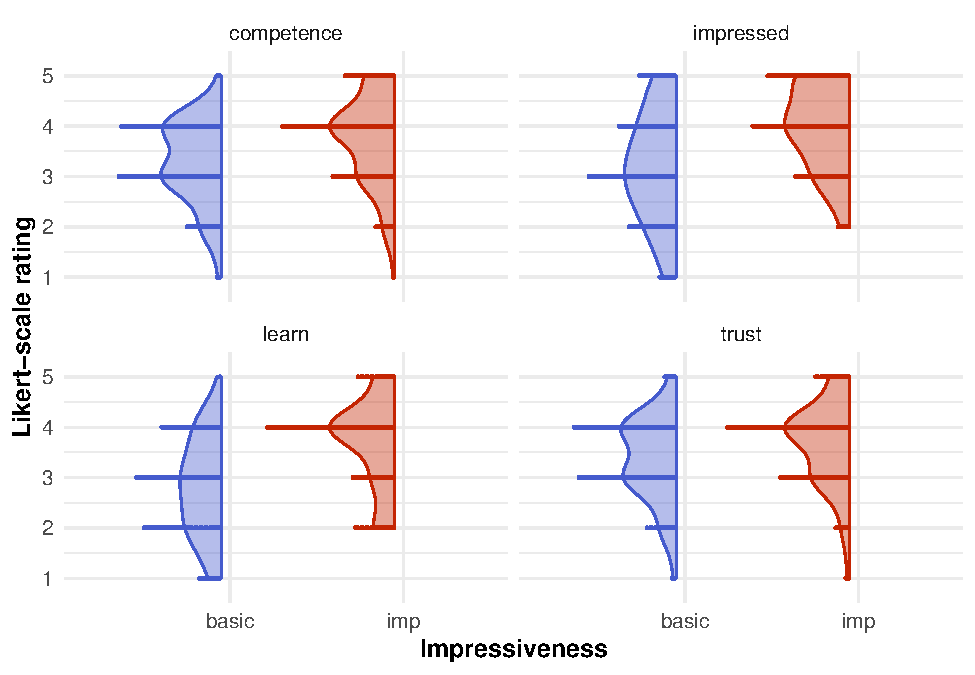
\includegraphics[keepaspectratio]{output/figures/exp1-plot.pdf}}
\caption{\label{fig:exp1-plot}Overview of treatment effect on various outcomes}
\end{figure}

The results of the models from the hypotheses can be found in table \ref{tab:exp1-hypotheses-table}.

\begin{table}
\centering\centering
\caption{\label{tab:exp1-hypotheses-table}The results of the models for the hypotheses}
\centering
\resizebox{\ifdim\width>\linewidth\linewidth\else\width\fi}{!}{
\begin{tabular}[t]{lcccc}
\toprule
  & H1a (Competence) & H1b (Competence pooled) & H2a (Trust) & H2b (Trust pooled)\\
\midrule
(Intercept) & 3.263*** & 2.043*** & 3.354*** & 2.449***\\
 & (0.086) & (0.185) & (0.086) & (0.177)\\
impressivenessimp & 0.495*** &  & 0.323*** & \\
 & (0.091) &  & (0.077) & \\
impressed &  & 0.407*** &  & 0.296***\\
 &  & (0.048) &  & (0.045)\\
SD (Intercept id) & 0.565 & 0.409 & 0.657 & 0.551\\
SD (Observations) & 0.642 & 0.640 & 0.542 & 0.547\\
\midrule
Num.Obs. & 198 & 198 & 198 & 198\\
R2 Marg. & 0.078 & 0.254 & 0.035 & 0.147\\
R2 Cond. & 0.480 & 0.471 & 0.609 & 0.577\\
AIC & 491.4 & 458.1 & 467.9 & 446.7\\
BIC & 504.5 & 471.3 & 481.0 & 459.9\\
ICC & 0.4 & 0.3 & 0.6 & 0.5\\
RMSE & 0.53 & 0.56 & 0.43 & 0.44\\
\bottomrule
\multicolumn{5}{l}{\rule{0pt}{1em}+ p $<$ 0.1, * p $<$ 0.05, ** p $<$ 0.01, *** p $<$ 0.001}\\
\end{tabular}}
\end{table}

The results of the model from RQ1 and of the models from RQ2 (interaction between impressiveness and consensus on competence/trust) can be found in table \ref{tab:exp1-consensus-table}.

\begin{table}
\centering\centering
\caption{\label{tab:exp1-consensus-table}The results of the models for the research questions}
\centering
\resizebox{\ifdim\width>\linewidth\linewidth\else\width\fi}{!}{
\begin{tabular}[t]{lccccc}
\toprule
  & RQ 1 & H1a x Consensus & H1b x Consensus & H2a x Consensus & H2b x Consensus\\
\midrule
(Intercept) & 2.768*** & 2.904*** & 1.899** & 3.287*** & 2.965***\\
 & (0.095) & (0.346) & (0.647) & (0.375) & (0.681)\\
impressivenessimp & 0.889*** & 0.132 &  & -0.371 & \\
 & (0.110) & (0.398) &  & (0.456) & \\
consensus &  & 0.117 & 0.153 & -0.006 & -0.250\\
 &  & (0.087) & (0.168) & (0.095) & (0.179)\\
impressivenessimp × consensus &  & 0.054 &  & 0.230+ & \\
 &  & (0.103) &  & (0.118) & \\
impressed &  &  & 0.391* &  & 0.129\\
 &  &  & (0.187) &  & (0.194)\\
impressed × consensus &  &  & -0.027 &  & 0.074\\
 &  &  & (0.048) &  & (0.050)\\
SD (Intercept id) & 0.535 & 0.634 & 0.552 & 0.547 & 0.390\\
SD (Observations) & 0.775 & 0.548 & 0.548 & 0.641 & 0.648\\
\midrule
Num.Obs. & 198 & 198 & 198 & 198 & 198\\
R2 Marg. & 0.183 & 0.056 & 0.155 & 0.101 & 0.262\\
R2 Cond. & 0.447 & 0.596 & 0.581 & 0.480 & 0.458\\
AIC & 539.3 & 473.5 & 457.3 & 495.0 & 467.7\\
BIC & 552.4 & 493.2 & 477.0 & 514.7 & 487.4\\
ICC & 0.3 & 0.6 & 0.5 & 0.4 & 0.3\\
RMSE & 0.67 & 0.43 & 0.44 & 0.53 & 0.57\\
\bottomrule
\multicolumn{6}{l}{\rule{0pt}{1em}+ p $<$ 0.1, * p $<$ 0.05, ** p $<$ 0.01, *** p $<$ 0.001}\\
\end{tabular}}
\end{table}

\clearpage

\section{Experiment 2b}\label{exp2b}

This experiment is not reported in the main article. Please note that on the OSF, all files related to this experiment are listed under ``experiment\_3'', as this corresponded to the order in which our different experiments were run.

\subsection{Difference with Experiment 2}\label{difference-with-experiment-2}

\FloatBarrier

In contrast to Experiment 3, we used a more direct recall measure---an open-ended text answer---and an even shorter time lag.

In Experiment 3, we quizzed participants about impressive scientific findings, either immediately after learning about them or after having gone through a distraction task. However, people's quiz performance did not vary between conditions--possibly because the quiz was generally too easy, and those questions which weren't easy were already hard to answer immediately after having read the text. In Experiment 4, we used a different design to overcome some of these issues.

Experiments 1 and 2 have shown that exposure to impressive scientific content can increase trust in science and perceived competence of scientists. In Experiment 3, we test if these impressions persist, and if they persists more than specific knowledge about the content.

The deficit model suggests that people do not trust science (enough), because they do not know enough about it. Accordingly, more knowledge about science generates trust. Here, we want to contrast this model with an alternative one: the trust-by-impression account. According to this model, people trust science at time T+1 not so much because they know about it at time T+1, but because they have been impressed by it at time T. We expected people to forget quickly about precise content, but that the impressions they gain about scientists' trustworthiness persist. We therefore predicted that our treatment - a short distraction task - will result in a stronger decrease of knowledge than a decreas in trust/impressiveness/competence.

H1: The difference in knowledge performance between treatment and control group is larger (more negative) than the difference in \ldots{}

\begin{itemize}
\item
  H1a: \ldots trust.
\item
  H1b: \ldots impressiveness.
\item
  H1c: \ldots competence.
\end{itemize}

\subsection{Methods}\label{methods-3}

\subsubsection{Participants}\label{participants-3}

We ran a power simulation to inform our choice of sample size. The power simulation suggested that with 150 participants, we would cross the power threshold of 90\% for the interaction effect (power = 0.958). Due to uncertainty about our parameters for the simulations, and because our budget allowed for it, we aimed to recruit a sample of 200 participants. We ended up with a sample of 202 participants (101 female, 100 male; \(age_\text{mean}\): 42.33, \(age_\text{sd}\): 13.74, \(age_\text{median}\): 41), none of which failed our attention check.

\subsubsection{Attention check}\label{attention-check-2}

Imagine you are playing video games with a friend and at some point your friend says: ``I don't want to play this game anymore! To make sure that you read the instructions, please write the three following words''I pay attention'' in the box below. I really dislike this game, it's the most overrated game ever.''

Do you agree with your friend? (Yes/No)

We excluded all participants whose answer did not resemble ``I pay attention''.

\subsubsection{Procedure}\label{procedure-3}

All participants read one vignette, established as impressive and trust enhancing in previous experiments. We randomized whether this vignette was about archaeology or entomology. Right after reading the vignette, all participants answered four seemingly relevant questions about the vignette, but which are of no interest to our hypotheses. The aim of these questions was to make the following distraction task for the treatment group less obvious.

For these decoy questions, we asked participants how clear the text was {[}1 - Not clear at all, 2 - Not very clear, 3 - Neither clear nor not clear, 4 - Quite clear, 5 - Very clear{]}, if the text presented any new or surprising information to them {[}1 - None at all, 2 - Very little, 3 - Moderately, 4 - Quite a bit, 5 - A significant amount{]}, if it made them think of archaeologists/entomologists as more knowledgeable than they thought before {[}1 - Strongly disagree, 2 - Disagree, 3 - Neither agree nor disagree, 4 - Agree, 5 - Strongly agree{]} and how much they felt they have learned about human history/insects by reading the text {[}1 - Nothing, 2 - A bit, 3 - Some, 4 - Quite a bit, 5 - A lot{]}.

Participants were randomly assigned to one of two groups: In the control group, participants proceeded immediately to answer all outcome questions. In the treatment group, participants engaged in a 5min distraction task before proceeding to the same outcome questions (Check how much longer these participants actually took on average). The distraction task consisted of reading two vignettes that were completely unrelated and answering a couple of questions about them.

For our outcomes, similar to previous experiments, we asked participants how impressed they were by the content (``How impressive do you think the findings of the archaeologists/entomologists described in the text are?'' {[}1 - Not impressive at all, 2 - Not very impressive, 3 - Neither impressive nor not impressive, 4 - Quite impressive, 5 - Very impressive{]}), how competent they believed the scientists of the discipline to be (``How competent do you think archaeologists/entomologists are?'' {[}1 - Not competent at all, 2 - Not very competent, 3 - Neither competent nor not competent, 4 - Quite competent, 5 - Very competent{]}), and how much they trusted the discipline (``How much would you trust the discipline of archaeologists/entomologists ?'' {[}1 - Not trust them at all, 2 - Not trust them much, 3 - Neither trust them or not trust them, 4 - Trust them quite a bit, 5 - Trust them a lot{]}).

To measure the retained knowledge about the content of the vignettes, we asked participants to answer 5 multiple choice questions (Table \ref{tab:exp2b-knowledge}). For each question, participants got 1 point for the correct answer, and 0 points for any other answer. We calculated an overall knowledge score as the sum of points for all five questions, such that the maximum score is 5 and the minimum score is 0. Whether participants first answered the quiz or the other outcome questions was randomized, in both the control and the treatment group

\subsubsection{Materials}\label{materials-4}

As in Experiment 2, Experiment 3 relied on the impressive version of the stimuli of Experiment 1 (see Table \ref{tab:exp1-stimuli}).

\begingroup\fontsize{8}{10}\selectfont

\begin{longtable}[t]{>{\raggedright\arraybackslash}p{25em}|>{\raggedright\arraybackslash}p{25em}}
\caption{\label{tab:exp2b-knowledge}Knowledge questions used in Experiment 3}\\
\toprule
Archaeology & Entomology\\
\midrule
\endfirsthead
\caption[]{\label{tab:exp2b-knowledge}Knowledge questions used in Experiment 3 \textit{(continued)}}\\
\toprule
Archaeology & Entomology\\
\midrule
\endhead

\endfoot
\bottomrule
\endlastfoot
According to the text, what can archaeologists determine from examining bones? 
a) Gender, age, and past diseases 
b) Gender, age, and handedness
c) Gender and age
d) Gender, age, past diseases, and handedness
(correct answer: a) & Which techniques have entomologists used to study flies' visual perception?
a) Sonar imaging
b) Electron microscopy 
c) X-ray diffraction 
d) Mass spectrometry
(correct answer: b)\\
 \vphantom{3} \vphantom{2} \vphantom{1} & \\
According to the text, how do archaeologists determine at what age someone stopped drinking their mother’s milk?
a) By analyzing their bones 
b) By examining their hair 
c) By studying their teeth 
d) By observing their burial rituals
(correct answer: c) & What is the order or magnitude of the shorter displays flies can perceive?
a) Picoseconds
b) Nanoseconds
c) Microseconds
d) Milliseconds
(correct answer: d)\\
 & \\
The text mentions nerves that are particularly enlarged in humans compared to apes, which are they? 
a) The nerves that control fine hand movements
b) The nerves that control breathing
c) The nerves that balance for bipedal motion
d) The nerves that control the digestive system
(correct answer: b) & Where are the sensitive hairs found on crickets located?
a) Legs  
b) Wings  
c) Rear  
d) Head  
(correct answer: \vphantom{1} c)\\
\addlinespace
 & \\
Why is the canal containing a nerve going from the brain to the thorax enlarged in Neanderthals? 
a) Because Neanderthals had a different diet
b) Because Neanderthals engaged in increased physical activity 
c) Because Neanderthals were left-handed 
d) Because Neanderthals were able to speak
(correct answer: d) & What technique did entomologists use to study the sensitivity of cricket hairs?
a) Mass spectrometry  
b) Electron microscopy  
c) Laser-Doppler velocimetry  
d) Sonar imaging  
(correct answer: c)\\
 & \\
According to the text, what evidence suggests that most Neanderthals were right-handed? 
a) Analysis of their bones 
b) Analysis of their tools 
c) Examination of their teeth 
d) Observation of their cave paintings
(correct answer: b) & According to the passage, how sensitive are the cricket hairs to air motion changes?
a) They react to changes equivalent to the energy of a single photon.  
b) They react to changes equivalent to the energy of a single atom.  
c) They react to changes equivalent to the energy of a single grain of sand.
d) They react to changes equivalent to the energy of a single breath.  
(correct answer: a)\\*
\end{longtable}
\endgroup{}

\subsection{Results and discussion}\label{results-and-discussion-3}

We tested these hypotheses with the following model:

\[
value = (\beta_{0} + b_\text{0, participant}) + \beta_{1} Treatment + \beta_{2} Outcome + \beta_{3} (Treatment \times Outcome) + \epsilon
\]

\[
b_\text{0, participant} \sim \mathcal{N}(0, \sigma^2_{participant})
\]

In this model, the dependent variable ``value'' represents a standardized version of the outcome variables. The variable ``Treatment'' is a binary indicator, where a value of 1 signifies that participants were exposed to the decoy (treatment group) and a value of 0 indicates that they were not (control group). The ``Outcome'' variable is also binary, distinguishing outcome measures: a value of 1 represents knowledge, while a value of 0 represents (in different models) one of the other outcomes, i.e.~trust, impressiveness, or competence. The interaction term (``Treatment x Outcome'') captures the difference in the treatment effect between these outcome measures. For example, a statistically significant, negative interaction coefficient would indicate that the difference between control and decoy group was larger for the knowledge measure than for trust/competence/impressiveness. Random intercepts for participants (\(b_\text{0, participant}\)) are included in the model to account for individual variability. These random intercepts are assumed to follow a normal distribution with a variance of \(\sigma^2_{participant}\).

Analyzing the effects of our treatment on all outcome variables of interest separately, we do not find evidence that our treatment affected any of them at all (\(\hat{b}_{\text{knowledge}}\) = -0.22 {[}-0.501, 0.052{]}, p = 0.111; \(\hat{b}_{\text{trust}}\) = 0.14 {[}-0.134, 0.421{]}, p = 0.309; \(\hat{b}_{\text{impressiveness}}\) = -0.22 {[}-0.494, 0.059{]}, p = 0.123; \(\hat{b}_{\text{competence}}\) = -0.09 {[}-0.37, 0.186{]}, p = 0.514). In other words, over a 5min distraction task, knowledge persisted, and so did perceptions of the scientific disciplines and the scientists.

Unsurprisingly, we do therefore not find evidence for our hypotheses, namely that our treatment--the distraction task--affected knowledge more than it did any of the other outcome variables (\(\hat{b}_{\text{trust}}\) = -0.37 {[}-0.759, 0.023{]}, p = 0.065; \(\hat{b}_{\text{impressiveness}}\) = -0.01 {[}-0.389, 0.375{]}, p = 0.972; \(\hat{b}_{\text{competence}}\) = -0.13 {[}-0.515, 0.251{]}, p = 0.497).

Table \ref{tab:exp2b-descriptives} provides a descriptive table of the results, and Figure \ref{fig:exp2b-plot} illustrates them. The results of the models from the hypotheses can be found in table \ref{tab:exp2b-hypotheses-table}. The treatment effects by outcome can be found in table \ref{tab:exp2b-treatment-effects}.

\begin{table}
\centering\centering
\caption{\label{tab:exp2b-descriptives}Descriptives}
\centering
\resizebox{\ifdim\width>\linewidth\linewidth\else\width\fi}{!}{
\begin{tabular}[t]{llrrrr}
\toprule
discipline & treatment & n\_correct\_mean & impressed\_mean & competence\_mean & trust\_mean\\
\midrule
archeo & control & 3.51 & 4.29 & 4.51 & 4.14\\
archeo & distraction & 3.49 & 4.08 & 4.42 & 4.21\\
entom & control & 3.51 & 4.17 & 4.66 & 4.02\\
entom & distraction & 2.88 & 4.12 & 4.65 & 4.16\\
\bottomrule
\end{tabular}}
\end{table}



\begin{figure}
\centering
\pandocbounded{\includegraphics[keepaspectratio]{output/figures/exp2b-plot.pdf}}
\caption{\label{fig:exp2b-plot}Overview of treatment effect on various outcomes}
\end{figure}

\begin{table}
\centering\centering
\caption{\label{tab:exp2b-hypotheses-table}Models for interaction hypotheses}
\centering
\resizebox{\ifdim\width>\linewidth\linewidth\else\width\fi}{!}{
\begin{tabular}[t]{lccc}
\toprule
  & Competence & Trust & Impressiveness\\
\midrule
(Intercept) & 0.047 & -0.074 & 0.112\\
 & (0.101) & (0.101) & (0.101)\\
treatmentdistraction & -0.092 & 0.144 & -0.217\\
 & (0.141) & (0.141) & (0.140)\\
outcome\_binary & 0.068 & 0.189 & 0.004\\
 & (0.139) & (0.143) & (0.139)\\
treatmentdistraction × outcome\_binary & -0.132 & -0.368+ & -0.007\\
 & (0.194) & (0.199) & (0.194)\\
SD (Intercept id) & 0.213 & 0.000 & 0.215\\
SD (Observations) & 0.976 & 0.998 & 0.973\\
\midrule
Num.Obs. & 404 & 404 & 404\\
R2 Marg. & 0.007 & 0.009 & 0.012\\
R2 Cond. & 0.052 &  & 0.058\\
AIC & 1164.2 & 1164.0 & 1162.2\\
BIC & 1188.2 & 1188.0 & 1186.3\\
ICC & 0.0 &  & 0.0\\
RMSE & 0.95 & 0.99 & 0.95\\
\bottomrule
\multicolumn{4}{l}{\rule{0pt}{1em}+ p $<$ 0.1, * p $<$ 0.05, ** p $<$ 0.01, *** p $<$ 0.001}\\
\end{tabular}}
\end{table}

\begin{table}
\centering\centering
\caption{\label{tab:exp2b-treatment-effects}Treatment effects by outcome}
\centering
\resizebox{\ifdim\width>\linewidth\linewidth\else\width\fi}{!}{
\begin{tabular}[t]{lcccc}
\toprule
  & Knowledge & Trust & Impressiveness & Competence\\
\midrule
(Intercept) & 0.115 & -0.074 & 0.112 & 0.047\\
 & (0.101) & (0.101) & (0.101) & (0.101)\\
treatmentdistraction & -0.224 & 0.144 & -0.217 & -0.092\\
 & (0.140) & (0.141) & (0.140) & (0.141)\\
\midrule
Num.Obs. & 202 & 202 & 202 & 202\\
R2 & 0.013 & 0.005 & 0.012 & 0.002\\
R2 Adj. & 0.008 & 0.000 & 0.007 & -0.003\\
AIC & 575.7 & 577.2 & 575.8 & 577.8\\
BIC & 585.6 & 587.1 & 585.8 & 587.7\\
Log.Lik. & -284.841 & -285.599 & -284.919 & -285.909\\
RMSE & 0.99 & 0.99 & 0.99 & 1.00\\
\bottomrule
\multicolumn{5}{l}{\rule{0pt}{1em}+ p $<$ 0.1, * p $<$ 0.05, ** p $<$ 0.01, *** p $<$ 0.001}\\
\end{tabular}}
\end{table}

\clearpage

\section{Experiment 2}\label{exp2}

\FloatBarrier

This is the experiment reported as Experiment 2 in the main article. Please note that on the OSF, all files related to this experiment are listed under ``experiment\_4'', as this corresponded to the order in which our different experiments were run.

This appendix only contains the attention check, as all analyses that were run are reported in the main article.

\subsection{Attention check}\label{attention-check-3}

Participants answered the following attention check: ``Please answer `Strongly agree' to this question to show you are paying attention. {[}1. Strongly disagree; 2. Somewhat disagree; 3. Neither agree nor disagree; 4. Somewhat agree; 5. Strongly agree{]}''. We excluded all participants who did not select ``5. Strongly agree''.


\end{document}
